\documentclass{wissdoc}
% Autor: Roland Bless 1996-2009, bless <at> kit.edu
% ----------------------------------------------------------------
% Hauptdokument
% ----------------------------------------------------------------
%%
%% $Id: thesis.tex 65 2012-05-10 10:32:11Z bless $
%%
%
% Zum Erstellen zweiseitiger PDFs (für Buchdruck) in der Datei "wissdoc.cls" folgende Zeile abändern:
%
% \LoadClass[a4paper,12pt,oneside]{book} % diese Klasse basiert auf ``book''
% in
%\LoadClass[a4paper,12pt,titlepage]{book} % diese Klasse basiert auf ``book''
%
%
% wissdoc Optionen: draft, relaxed, pdf --> siehe wissdoc.cls
% ------------------------------------------------------------------
% Weitere packages: (Dokumentation dazu durch "latex <package>.dtx")
\usepackage[numbers,sort&compress]{natbib}
% \usepackage{varioref}
% \usepackage{float}    %z.B. \floatstyle{ruled}\restylefloat{figure}
% \usepackage{subfigure}
% \usepackage{fancybox} % für schattierte,ovale Boxen etc.
% \usepackage{tabularx} % automatische Spaltenbreite
% \usepackage{supertab} % mehrseitige Tabellen
% \usepackage[svnon,svnfoot]{svnver} % SVN Versionsinformation 
\usepackage{amsmath,amsthm,amssymb}
\usepackage[ruled,vlined,linesnumbered]{algorithm2e}
\usepackage{graphicx}
\usepackage{hyperref}
\usepackage{makecell}
\usepackage{pgfplots}
\usepackage{verbatim}
\usepackage[width=.75\textwidth]{caption}
\usepackage{listings}
\usepackage{hhline}
\usepackage{wrapfig}
\usepackage{mathtools}
\usepackage{subcaption}
%% ---------------- end of usepackages -------------

\newcommand\mycommfont[1]{\footnotesize{\textit{#1}}}
\SetCommentSty{mycommfont}
\SetKwComment{Comment}{(}{)}



\colorlet{punct}{red!60!black}
\definecolor{background}{HTML}{EEEEEE}
\definecolor{delim}{RGB}{20,105,176}
\colorlet{numb}{magenta!60!black}

\lstdefinelanguage{json}{
    basicstyle=\scriptsize\ttfamily,  
    numbers=left,
    numberstyle=\scriptsize,
    stepnumber=1,
    numbersep=8pt,
    showstringspaces=false,
    breaklines=true,
    frame=lines,
    backgroundcolor=\color{background},
    literate=
     *{0}{{{\color{numb}0}}}{1}
      {1}{{{\color{numb}1}}}{1}
      {2}{{{\color{numb}2}}}{1}
      {3}{{{\color{numb}3}}}{1}
      {4}{{{\color{numb}4}}}{1}
      {5}{{{\color{numb}5}}}{1}
      {6}{{{\color{numb}6}}}{1}
      {7}{{{\color{numb}7}}}{1}
      {8}{{{\color{numb}8}}}{1}
      {9}{{{\color{numb}9}}}{1}
      {:}{{{\color{punct}{:}}}}{1}  
      {,}{{{\color{punct}{,}}}}{1}
      {\{}{{{\color{delim}{\{}}}}{1}
      {\}}{{{\color{delim}{\}}}}}{1}
      {[}{{{\color{delim}{[}}}}{1}
      {]}{{{\color{delim}{]}}}}{1},
}

\lstdefinestyle{cpp}{
basicstyle=\ttfamily\footnotesize,
morekeywords={HOTM,num,numint},
captionpos=b,
xleftmargin=15pt,
numbers=left,
stepnumber=1
}

%\svnversion{$Id: thesis.tex 65 2012-05-10 10:32:11Z bless $} % In case that you want to include version information in the footer

%% Informationen für die PDF-Datei
\hypersetup{
 pdfauthor={Benedikt Lüken-Winkels},
 pdftitle={Masterarbeit}
 pdfsubject={Untersuchungen zur Henon Iteration},
 pdfkeywords={Masterarbeit}
}

% Macros, nicht unbedingt notwendig
%%%%%%%%%%%%%%%%%%%%%%%%%%%%%%%%%%%%%%%%%%%%%%%%%%%%%%%%%%
% macros.tex -- einige mehr oder weniger nuetzliche Makros
% Autor: Roland Bless 1998
%%%%%%%%%%%%%%%%%%%%%%%%%%%%%%%%%%%%%%%%%%%%%%%%%%%%%%%%%%
% $Id: macros.tex 33 2007-01-23 09:00:59Z bless $
%%%%%%%%%%%%%%%%%%%%%%%%%%%%%%%%%%%%%%%%%%%%%%%%%%%%%%%%%%


%%%%%%%%%%%%%%%%%%%%%%%
% Kommentare 
%%%%%%%%%%%%%%%%%%%%%%%
\ifnotdraftelse{
\newcommand{\Kommentar}[1]{}
}{\newcommand{\Kommentar}[1]{{\em #1}}}
% Alles innerhalb von \Hide{} oder \ignore{} 
% wird von LaTeX komplett ignoriert (wie ein Kommentar)
\newcommand{\Hide}[1]{}
\let\ignore\Hide

%%%%%%%%%%%%%%%%%%%%%%%%%
% Leere Seite ohne Seitennummer, wird aber gezaehlt
%%%%%%%%%%%%%%%%%%%%%%%%%

\newcommand{\leereseite}{% Leerseite ohne Seitennummer, nächste Seite rechts (wenn 2-seitig)
 \clearpage{\pagestyle{empty}\cleardoublepage}
}
%%%%%%%%%%%%%%%%%%%%%%%%%%
% Flattersatz rechts und Silbentrennung, Leerraum nach rechts maximal 1cm
%%%%%%%%%%%%%%%%%%%%%%%%%%
\makeatletter
\newcommand{\myraggedright}{%
 \let\\\@centercr\@rightskip 0pt plus 1cm
 \rightskip\@rightskip
  \leftskip\z@skip
  \parindent\z@
  \spaceskip=.3333em
  \xspaceskip=.5em}
\makeatother

\makeatletter
\newcommand{\mynewline}{%
 \@centercr\@rightskip 0pt plus 1cm
}
\makeatother


%%%%%%%%%%%%%%%%%%%%%%%%%%
% Für Index
%%%%%%%%%%%%%%%%%%%%%%%%%%
\makeatletter
\def\mydotfill{\leavevmode\xleaders\hb@xt@ .44em{\hss.\hss}\hfill\kern\z@}
\makeatother
\def\bold#1{{\bfseries #1}}
\newbox\dbox \setbox\dbox=\hbox to .4em{\hss.\hss} % dot box for leaders
\newskip\rrskipb \rrskipb=.5em plus3em % ragged right space before break
\newskip\rrskipa \rrskipa=-.17em plus -3em minus.11em % ditto, after
\newskip\rlskipa \rlskipa=0pt plus3em % ragged left space after break
\newskip\rlskipb \rlskipb=.33em plus-3em minus.11em % ragged left before break
\newskip\lskip \lskip=3.3\wd\dbox plus1fil minus.3\wd\dbox % for leaders
\newskip \lskipa \lskipa=-2.67em plus -3em minus.11em %after leaders
\mathchardef\rlpen=1000 \mathchardef\leadpen=600
\def\rrspace{\nobreak\hskip\rrskipb\penalty0\hskip\rrskipa}
\def\rlspace{\penalty\rlpen\hskip\rlskipb\vadjust{}\nobreak\hskip\rlskipa}
\let\indexbreak\rlspace
\def\raggedurl{\penalty10000 \hskip.5em plus15em \penalty0 \hskip-.17em plus-15em minus.11em}
\def\raggeditems{\nobreak\hskip\rrskipb \penalty\leadpen \hskip\rrskipa %
\vadjust{}\nobreak\leaders\copy\dbox\hskip\lskip %
\kern3em \penalty\leadpen \hskip\lskipa %
\vadjust{}\nobreak\hskip\rlskipa}
\renewcommand*\see[2]{\rlspace\emph{\seename}~#1} % from makeidx.sty

%%%%%%%%%%%%%%%%%%%%%%%%%%
% Neue Seite rechts, leere linke Seite ohne Headings
%%%%%%%%%%%%%%%%%%%%%%%%%%
\newcommand{\xcleardoublepage}
{{\pagestyle{empty}\cleardoublepage}}

%%%%%%%%%%%%%%%%%%%%%%%%%%
% Tabellenspaltentypen (benoetigt colortbl)
%%%%%%%%%%%%%%%%%%%%%%%%%%
\newcommand{\PBS}[1]{\let\temp=\\#1\let\\=\temp}
\newcolumntype{y}{>{\PBS{\raggedright\hspace{0pt}}}p{1.35cm}}
\newcolumntype{z}{>{\PBS{\raggedright\hspace{0pt}}}p{2.5cm}}
\newcolumntype{q}{>{\PBS{\raggedright\hspace{0pt}}}p{6.5cm}}
\newcolumntype{g}{>{\columncolor[gray]{0.8}}c} % Grau
\newcolumntype{G}{>{\columncolor[gray]{0.9}}c} % helleres Grau

%%%%%%%%%%%%%%%%%%%%%%%%%%
% Anführungszeichen oben und unten
%%%%%%%%%%%%%%%%%%%%%%%%%%
\newcommand{\anf}[1]{`{#1}'}

%%%%%%%%%%%%%%%%%%%%%%%%%%
% Tiefstellen von Text
%%%%%%%%%%%%%%%%%%%%%%%%%%
% S\tl{0} setzt die 0 unter das S (ohne Mathemodus!)
% zum Hochstellen gibt es uebrigens \textsuperscript
\makeatletter
\DeclareRobustCommand*\textlowerscript[1]{%
  \@textlowerscript{\selectfont#1}}
\def\@textlowerscript#1{%
  {\m@th\ensuremath{_{\mbox{\fontsize\sf@size\z@#1}}}}}
\let\tl\textlowerscript
\let\ts\textsuperscript
\makeatother

%%%%%%%%%%%%%%%%%%%%%%%%%%
% Gauß-Klammern
%%%%%%%%%%%%%%%%%%%%%%%%%%
\newcommand{\ceil}[1]{\lceil{#1}\rceil}
\newcommand{\floor}[1]{\lfloor{#1}\rfloor}

%%%%%%%%%%%%%%%%%%%%%%%%%%
% Average Operator (analog zu min, max)
%%%%%%%%%%%%%%%%%%%%%%%%%%
\def\avg{\mathop{\mathgroup\symoperators avg}}

%%%%%%%%%%%%%%%%%%%%%%%%%%
% Wortabkürzungen
%%%%%%%%%%%%%%%%%%%%%%%%%%
\def\zB{z.\,B.\ }
\def\dh{d.\,h.\ }
\def\ua{u.\,a.\ }
\def\su{s.\,u.\ }
\newcommand{\bzw}{bzw.\ }

%%%%%%%%%%%%%%%%%%%%%%%%%%%%%%%%%%%
% Einbinden von Graphiken
%%%%%%%%%%%%%%%%%%%%%%%%%%%%%%%%%%%
% global scaling factor
\def\gsf{0.9}
%% Graphik, 
%% 3 Argumente: Datei, Label, Unterschrift
\newcommand{\Abbildung}[3]{%
\begin{figure}[tbh] %
\centerline{\scalebox{\gsf}{\includegraphics*{#1}}} %
\caption{#3} %
\label{#2} %
\end{figure} %
}
\let\Abb\Abbildung
%% Abbps
%% Graphik, skaliert, Angabe der Position
%% 5 Argumente: Position, Breite (0 bis 1.0), Datei, Label, Unterschrift
\newcommand{\Abbildungps}[6]{%
\begin{figure}[#1]%
\begin{center}
\scalebox{\gsf}{\includegraphics*[width=#2\textwidth]{#3}}%
\caption[#5]{#6}%
\label{#4}%
\end{center}
\end{figure}%
}
\let\Abbps\Abbildungps
%% Graphik, Angabe der Position, frei wählbares Argument für includegraphics
%% 5 Argumente: Position, Optionen, Datei, Label, Unterschrift
\newcommand{\Abbildungpf}[5]{%
\begin{figure}[#1]%
\begin{center}
\scalebox{\gsf}{\includegraphics*[#2]{#3}}%
\caption{#5}%
\label{#4}%
\end{center}
\end{figure}%
}
\let\Abbpf\Abbildungpf

%%
% Anmerkung: \resizebox{x}{y}{box} skaliert die box auf Breite x und Höhe y,
%            ist x oder y ein !, dann wird das usprüngliche 
%            Seitenverhältnis beibehalten.
%            \rescalebox funktioniert ähnlich, nur das dort ein Faktor
%            statt einer Dimension angegeben wird.
%%
% \Abbps{Position}{Breite in Bruchteilen der Textbreite}{Dateiname}{Label}{Bildunterschrift}
%

\newcommand{\refAbb}[1]{%
s.~Abbildung \ref{#1}}

\newcommand{\e}{\'{e}}

%%%%%%%%%%%%%%%%%%%%
%% end of macros.tex
%%%%%%%%%%%%%%%%%%%%


% Print URLs not in Typewriter Font
\def\UrlFont{\rm}

\newcommand{\blankpage}{% Leerseite ohne Seitennummer, nächste Seite rechts
 \clearpage{\pagestyle{empty}\cleardoublepage}
}

%% Einstellungen für das gesamte Dokument

% Trennhilfen
% Wichtig! 
% Im ngerman-paket sind zusätzlich folgende Trennhinweise enthalten:
% "- = zusätzliche Trennstelle
% "| = Vermeidung von Ligaturen und mögliche Trennung (bsp: Schaf"|fell)
% "~ = Bindestrich an dem keine Trennung erlaubt ist (bsp: bergauf und "~ab)
% "= = Bindestrich bei dem Worte vor und dahinter getrennt werden dürfen
% "" = Trennstelle ohne Erzeugung eines Trennstrichs (bsp: und/""oder)

% Trennhinweise fuer Woerter hier beschreiben
\hyphenation{
% Pro-to-koll-in-stan-zen
}

% Index-Datei öffnen
\ifnotdraft{\makeindex}

\begin{document}
\renewcommand{\ttdefault}{pcr}
\frontmatter
\pagenumbering{roman}
\ifnotdraft{
 %% Titelseite
%% Vorlage $Id: titelseite.tex 61 2012-05-03 13:58:03Z bless $

\def\usesf{}
\let\usesf\sffamily % diese Zeile auskommentieren für normalen TeX Font

\newsavebox{\Erstgutachter}
\savebox{\Erstgutachter}{\usesf xxxxxxxxxx}
\newsavebox{\Zweitgutachter}
\savebox{\Zweitgutachter}{\usesf xxxxxxxxxx}
\newsavebox{\Betreuer}
\savebox{\Betreuer}{\usesf xxxxxxxxxx}

\begin{titlepage}
\setlength{\unitlength}{1pt}
\begin{picture}(0,0)(85,770)
%\includegraphics[width=\paperwidth]{logos/KIT_Deckblatt}
\end{picture}

\thispagestyle{empty}

%\begin{titlepage}
%%\let\footnotesize\small \let\footnoterule\relax
\begin{center}
\hbox{}
\vfill
{\usesf
{\huge\bfseries Implementierung nichtlinearer Taylormodelle \par}
\vskip 1.8cm
{\huge Forschungspraktikum}\\


{\large Universität Trier\\
FB IV - Informatikwissenschaften\\
Professur Arithmetische Algorithmen\\}

\vskip 3cm
\begin{tabular}{p{3cm}l}
Betreuer: & apl. Prof. Dr.  Norbert Müller \\
\end{tabular}
\vskip 3cm
Vorgelegt am xx.xx.xxxx von:\\
\vskip .5cm
Benedikt Lüken-Winkels\\
Baltzstraße 6\\
54296 Trier\\
s4beluek@uni-trier.de\\
Matr.-Nr. 1138844
}
\end{center}
\vfill
\end{titlepage}
%% Titelseite Ende


%%% Local Variables: 
%%% mode: latex
%%% TeX-master: "thesis"
%%% End: 

 %\blankpage % Leerseite auf Titelrückseite
 \chapter*{Zusammenfassung}
%% ==============================
In dieser Arbeit wurde die Verwendung nichtlinearer Taylormodelle in der Praxis anhand der zweidimensionalen H\e non-Abbildung untersucht. Die Anwendung spezieller Operationen auf den Taylormodellen und die Verwendung der reellen Zahlen der \verb+iRRAM+-Softwarebibliothek ergibt eine vielzahl an Konfigurationsmöglichkeiten, welche experimentell verglichen und evaluiert wurden, um eine möglichst optimale Belegung der Parameter zu finden.

Der Quellcode des im Zuge der Arbeit entstandenen Programms \verb+HOTM+ (\textit{High Order Taylor Model}) ist Online\footnote{\url{https://gitlab.rlp.net/s4beluek/hotaylormodels} (Stand 30.03.21)} und auf einem der Arbeit beigelegten Datenträger verfügbar.
  
}
%
%% *************** Hier geht's ab ****************
%% ++++++++++++++++++++++++++++++++++++++++++
%% Verzeichnisse
%% ++++++++++++++++++++++++++++++++++++++++++
\ifnotdraft{
{\parskip 0pt\tableofcontents} % toc bitte einzeilig
%\blankpage
\listoffigures
%\blankpage
\listoftables
%\blankpage
\lstlistoflistings
}


%% ++++++++++++++++++++++++++++++++++++++++++
%% Hauptteil
%% ++++++++++++++++++++++++++++++++++++++++++
\graphicspath{{img/}}

\mainmatter
\pagenumbering{arabic}
%% Einleitung.tex
%% $Id: einleitung.tex 61 2012-05-03 13:58:03Z bless $
%%

\chapter{Einleitung}
\label{ch:Einleitung}
%% ==============================

Das Rechnen mit reellen Zahlen und Funktionen auf denselben bedeutet die Verarbeitung einer unendlichen Menge an Informationen, die in der computergestützten Praxis lediglich mit einer endlichen Approximation beschrieben werden können \cite{Brattka2008}. Eine solche Beschränkung hat zu Folge, dass arithmetische Operationen keine exakten Ergebnisse ohne Fehler liefern. Dieser wird in der Disziplin der \textit{Exakten Reellen Arithmetik} durch Intervalle abgeschätzt, die den tatsächlichen Wert mitsamt Rundungsfehler umschließen und so ein korrektes Ergebnis garantieren können. Eine entsprechende Implementierung bietet die \verb.C++.-Softwarebibliothek \verb+iRRAM+ \cite{Mller2009EnhancingIE}, die reelle Zahlen zu einer beliebigen Genauigkeit, statt der häufig verwendetet \textit{double}-Präzision, annähert.
Jedoch entsteht durch die so betriebene Intervallarithmetik das Problem der Überschätzung des Wertebereichts, zum Beispiel beim mehrfachen Auftreten derselben Variable in einem Term. Ein weit verbreiteter Lösungsansatz ist die Verwendung von Taylormodellen, mit denen Zahlen als höherdimensionale Polynome mit reellen Koeffizienten und einem Fehlerintervall dargestellt werden \cite{DBLP:conf/macis/BrausseKM15} \cite{makino2001}. Zudem speichern Variablen (\anf{Fehlersymbole}) die Rechenfehler und deren Abhängigkeitsinformationen. Eine leicht veränderte Version der Taylormodelle wird im \verb.C++.-Programm \verb+Tangentspace+\footnote{\url{http://informatik.uni-trier.de/~mueller/Research/Tangentspace/} (Stand 29.03.2021)} implementiert. Die Taylormodelle bestehen hier aus linearen Polynomen mit beliebigen Intervallkoeffizienten und rationalen Endpunkten. Die Taylomodelle werden verwendet, um lineare Schranken für nichtlineare Funktionen zu bestimmen. Eine weitere Implementierung von Brauße et al. \cite{DBLP:conf/macis/BrausseKM15} verwendet reelle Endpunkte für die Intervallkoeffizienten und die Intervalle der Fehlersymbole. Das im Rahmen dieser Arbeit enstandene \verb.C++.-Programm \verb+HOTM+ (\textit{High Order Taylor Model}) bildet eine Kombination aus diesen beiden Herangehensweisen, da Intervalle mit beliebigen reellen Endpunkten verwendet werden. 

\paragraph{Zielsetzung}

Ziel dieser Arbeit war die Untersuchung nichtlinearer Taylormodelle in der praktischen Anwendung. Hierzu wurde das \verb.C++.-Programm \verb+HOTM+ (\textit{High Order Taylor Model}), beziehungsweise der gleichnamige Zahlentyp implementiert. Die Taylormodelle bestehen aus Polynomen mit Intervallkoeffizienten, welche die reellen Zahlen der \verb+iRRAM+-Software-Bibilothek als Endpunkte verwenden. Mit den so definierten Taylormodellen und damit einer mehrstufigen Intervallarchitektur ergibt sich eine Vielzahl an Konfigurationsmöglichkeiten von der Breite der Endpunkte der Intervalle, bis hin zu abstrakteren Operationen auf den Taylormodellen. An Hand von Berechnungen der H\e non-Abblildung werden diese evaluiert und versucht, eine möglichst optimale Einstellung für die Parameter der \verb+HOTM+ im zweidimensionalen Raum ($\mathbb{R}^2$) zu finden.

\paragraph{Gliederung}

Als praktisch ausgelegt Arbeit liegt der Schwerpunkt bei der Implementierung und den damit erzeugten experimentellen Ergebnissen. Die Basis hierfür bilden die in Kapitel \ref{ch:Grundlagen} beschriebenen Grundlagen, welche sich in H\e non-Abbildung, Taylormodelle und Lyapunov Exponenten gliedern. Diese Überblicke sollen das Verständnis über Entscheidungen in der Implementierung, die Deutung der Grafiken und der Ergebnisse vereinfachen. In Kapitel \ref{ch:Implementierung} werden die implementierten Operationen und Algorithmen der \verb+HOTM+ beschrieben. Mit der Anwerndung bei der H\e non-Abbildung werden diese in Kapitel \ref{ch:Evaluierung} evaluiert und verschiedenene Konfigurationen verglichen. Während der Implementierung und Durchführung der Experimente sind weiterführende Ideen und Anwendungsmöglichkeiten für die \verb+HOTM+ entstanden, auf die im Ausblick in Kapitel \ref{ch:fazit} neben der Diskussion der Ergebnisse eingegangen wird.

\paragraph{Relevante Literatur}
Die für diese Arbeit relevante Literatur lässt sich in vier Kategorien aufteilen, vergleichbar mit den später eingeführten Abstraktionsebenen, die sich aus dem Aufbau der \verb+HOTM+ ergeben. Für die grundlegende Zahlendarstellung wir die Implementierung der reellen Zahlen der \verb+iRRAM+ von Müller verwendet. Funktionsweisen und mögliche Anpassungen der Software-Bibilothek können den Quellen \cite{Mller2009EnhancingIE} und  \cite{mueller2001} entnommen werden. Für eine theoretische Grundlage der hier praktisch angewendeten Berechenbaren Analysis wird auf ein Tutorial von Brattka et al. \cite{Brattka2008} verwiesen. Spandl untersucht in \cite{DBLP:spandl} mit Hilfe der \verb+iRRAM+ den Lyapunov Exponenten für dynamische Systeme und zieht dabei Intervallmethoden heran, was einen zentralen Teil dieser Arbeit darstellt. 

Da die \verb+HOTM+ auf der nächst höheren Ebene aus Polynomen mit Intervallkoeffizienten bestehen, wurde eine allgemeine Intervallarithmetik, wie im Standardwerk von Moore \cite{moore1979} beschrieben implementiert. Yan et al. führen in \cite{geobuckets} einen Algorithmus ein, der die Addition von Polynomen effizient gestaltet, welcher in \cite{geobucketsmulti} für die Multiplikation formuliert ist. Mit dieser Basis können die Taylormodelle, wie in \cite{makino2001} und \cite{DBLP:conf/macis/BrausseKM15} beschrieben, implementiert werden.

In \cite{DBLP:conf/macis/BrausseKM15} sind zudem weiterführende Operationen auf Taylormodellen zu finden. Diese werden unter anderem im Programm \verb+Tangentspace+, auf dem die \verb+HOTM+s aufbauen, verwendet und ermöglicht geometrische Lösungen für Konfliktgesteuerte Gleichungslöser. Die Funktionsweise der so implementierten Taylormodelle wird an Hand der H\e non-Abblildung untersucht. Hierzu existieren neben dem ursprünglichen Paper von M. H\e non \cite{henon1976}, viele Experimente und Untersuchungen, wie Oliviera et al., die sich in \cite{MartinsdeOliveira2020} mit verschiedenen Parameterbelegungen beschäftigen.






%%% Local Variables: 
%%% mode: latex
%%% TeX-master: "thesis"
%%% End: 
  % Einleitung
%% grundlagen.tex
%% $Id: grundlagen.tex 61 2012-05-03 13:58:03Z bless $
%%

\chapter{Grundlagen}
\label{ch:Grundlagen}
%% ==============================
\section{H\e non-Abbildung}
Die H\e non-Abbildung bietet eine Möglichkeit, das Verhalten eines seltsamen Attraktors (\textit{engl. \anf{strange attractor}}), wie dem des Lorenz Systems, mit einer recht einfachen Abbildung zu untersuchen.

Konviergieren die Werte einer Funktion in einem bestimmten Wertebereich $R$, der Fangzone (\textit{engl. \anf{trap zone}}), gegen einen Punkt oder eine Kurve, spricht man von einem Attraktor. Dieser Attraktor kann jedoch auch eine komplexere Struktur haben. Auf einem solchen seltsamen Attraktor springen die Werte hin und her und reagieren hochempfindlich auf Änderungen der Initialbedingungen. Dieses Verhalten lässt mit der Abbildung $x_{i+1}=y_i + 1- a x_i^2, y_{i+1} = bx_i$, bzw 
$$f(x,y) = (y + 1- a x^2,bx)$$
beobachten. $f$ erfüllt dieselben Kriterien, wie der durch eine dreidimensionale Differenzialgleichung entstehenden Lorenz-Attraktor, allerdings wurde $f$ so definiert, dass auch höhere Iterationszahlen leichter zu berechnen und zu analysieren sein sollen. Die H\e non-Abbildung bildet den $\mathbb{R}^2$ auf sich selbst ab. Dieser Vorgang besteht aus drei Schritten. Man betrachte eine Fläche entlang der $x$-Achse gelegen:

\textbf{Dehnen und Falten}
$$T': x'=x, y'= 1+ y - ax^2$$
Mit dem Parameter $a$ kann die Stärke der Biegung gesteuert werden.


\textbf{Kontrahieren}
$$T'': x''= b\cdot x, y''= y'$$
Ein $|b|<1$ bedeutet, dass sich die Fläche zusammen zieht. Wird $b$ zu groß gewählt, so entsteht eine zu große Kontraktion und der Attraktor ist schwerer erkennbar. Ist $b$ zu klein, ist der Effekt zu gering und das Verhalten der Abbildung ist nicht mehr chaotisch.


\textbf{Rotieren}
$$T''': x'''= y'', y'''= x''$$
Im letzten Schritt werden die Achsen vertauscht und somit dir Fläche um rotiert.


Die entstehende Abbildung hat unter Anderem folgende Eigenschaften:
\begin{itemize}
 \item Invertierbar: $(x_{n+1}, y_{n+1})$ kann eindeutig auf $(x_n, y_n)$ zurückgeführt werden.
 \item Kontrahiert Flächen: Mit $|b|<1$ werden Flächen kleiner.
 \item Besitzt eine Fangzone, die einen Attraktor enthält. Allerdings landen nicht immer alle Orbits in der Fangzone, da wegen $x^2$ Terme bestimmter Größe nach $\infty$ laufen können.
\end{itemize}


Abbildung \ref{fig:henonevo} zeigt die einzelnen Schritte einer Evolution der H\e non-Abbildung anhand eines Rechtecks, welches als nichtlineares Taylormodell definiert wurde.
$$x_0 = 0 + 1 \cdot \lambda_1 \hspace{.5cm} (\lambda_1 \in [0 \pm 0.4])$$
$$\ y_0 = 0 + 1 \cdot \lambda_2 \hspace{.5cm} (\lambda_2 \in [0 \pm 0.05])$$
Das Rechteck wird gedehnt und gefaltet, dann kontrahiert und zuletzt rotiert, beziehungsweise gespiegelt. 

\Abbildungps{tbh}{.7}{img/henon_evo.pdf}{fig:henonevo}{H\e non-Abbildung: Einfache Evolution}{Einfache Evolution der H\e non Abbildung, aufgeteilt in das initiale Rechteck und die drei Zwischenschritte.}

Für die Parameter $a=1.4$ und $b=0.3$ ergibt sich eine Fangzone in der sich die Funktionswerte auf einem seltsamen Attraktor bewegen. Das bedeutet, dass ein Punkt, in der Fangzone, beziehungsweise auf dem Attraktor liegt, wiederum auf diesen abgebildet wird. Der Attraktor ist in Abbildung \ref{fig:strangeattractor} zu sehen. Hier wurden, ausgehend vom Punkt $(0,0)$, 10000 Iterationen der H\e non-Abbildung berechnet und jeweils das Ergebnis eingezeichnet. Es ist deutlich erkennbar, dass sich der Attraktor teils nahe am Rande der Fangzone bewegt. Bereits bei einer leichten Überschätzung des Ergebnisses kann dies dazu führen, dass die Funktionswerte die Fangzone verlassen.

\Abbildungps{tbh}{.7}{img/attractor.pdf}{fig:strangeattractor}{H\e non-Abbildung: Attraktor}{Seltsamer Attraktor der H\e non-Abbildung für $a=1,4$ und $b=0.3$ mit 10000 Punkten.}

Mit fortlaufenden Interationen wird das Rechteck immer weiter verzerrt. In Abbildung \ref{fig:henonevocolored} ist der Farbkodierung folgend, der Ursprung der Regionen im Initalrechteck erkennbar.

\Abbildungps{tbh}{.7}{img/henon_evo_colored.pdf}{fig:henonevocolored}{H\e non-Abbildung: Einfache Evolution mit Farbkodierung}{Einfache Evolution der H\e non Abbildung, aufgeteilt in das initiale Rechteck und die drei Zwischenschritte mit Farbkodierung zur Rückführung der Regionen.}     


\Abbildungps{tbh}{.9}{img/7iter_w_sweep.pdf}{fig:7iter}{H\e non-Abbildung: Mehrere Iterationen mit Farbkodierung}{Mehrere Iterationen mit Farbkodierung}


%%% Local Variables: 
%%% mode: latex
%%% TeX-master: "thesis"
%%% End: 
 
  % Grundlagen
% %% analyse.tex
%% $Id: analyse.tex 61 2012-05-03 13:58:03Z bless $

\chapter{Analyse}
\label{ch:Analyse}
%% ==============================



%%% Local Variables: 
%%% mode: latex
%%% TeX-master: "thesis"
%%% End: 
     % Analyse
%% entwurf.tex
%% $Id: entwurf.tex 61 2012-05-03 13:58:03Z bless $
%%

\chapter{Entwurf / Konzeption}
\label{ch:Entwurf}
%% ==============================
In diesem Kapitel erfolgt die ausführliche Beschreibung des eigenen
Lösungsansatzes. Dabei sollten Lösungsalternativen diskutiert und
Entwurfsentscheidungen dargelegt werden.



%% ==============================
\section{Zusammenfassung}
%% ==============================
\label{ch:Entwurf:sec:zusammenfassung}

Am Ende sollten ggf. die wichtigsten Ergebnisse nochmal in \emph{einem}
kurzen Absatz zusammengefasst werden.

%%% Local Variables: 
%%% mode: latex
%%% TeX-master: "thesis"
%%% End: 
     % Entwurf
%% implemen.tex
%% $Id: implemen.tex 61 2012-05-03 13:58:03Z bless $
%%

\chapter{Implementierung}
\label{ch:Implementierung}
%% ==============================



\section{iRRAM}
\label{sec:irram}
Die Software-Bibliothek \verb+iRRAM+ \cite{Mller2009EnhancingIE} basiert auf Intervallen als Zahlentyp, um diese mit einer beliebigen Genauigkeit darstellen zu können. Zunächst wird mit Double-Präzision, also 64-Bit Zahlen gerechnet, welche verwendet werden, bis das Ergebnis für die angefragte Präzision nicht mehr genau ausgegeben werden kann, beziehungsweise bis zu einer bestimmten Anzahl an Bits. Ist dies der Fall, geschieht eine Iteration mit einer erhöhten Genauigkeit, also längeren Zahlen, welche dann mit Hilfe von \verb+MPFR+ dargestellt werden.
Für eine solche Iteration werden gerade so viele Zwischenergebnisse während der Berechnung gespeichert, dass eine Wiederholung der Schritte mit höherer Präzision möglich ist. Da nicht die gesamte Berechnung in jeder Iteration wiederholt wird, müssen während der Laufzeit Sichtbarkeit von Variablen und Zwischenergebnissen für den Nutzer genau kontrolliert und unter Umständen beschränkt werden, da sonst unerwartetes Verhalten und Exceptions entstehen können, indem die zugegriffenen Werte gegebenfalls nicht in der aktuellen Iteration existieren.


Einige der für rationale Zahlen zur Verfügung stehenden Funktionen, wie der Vergleich zweier Zahlen, sind mit reellen Zahlen nicht ohne weiteres Möglich. Dies gilt insbesondere für den Test auf Gleichheit und die Vorzeichenfunktion $sign$. Bei all diesen Funktionen handelt es sich im Reellen (und bei der \verb+iRRAM+) um mehrwertige Funktionen, da sich das jeweilige Ergebnis mit veränderter Präzsion in der Darstellung der Zahlen ändern kann. Dieses Problem wird in \verb+hotm+ durch den \verb+SignType+ adressiert. Zusätzlich zu den Werten 'positiv' (=\verb+POS+) und 'negativ' (=\verb+NEG+),  kann die Vorzeichenfunktion \verb+sign+ den Wert 'ambivalent' (=\verb+AMBI+) ausgeben, wenn nicht entscheidbar ist, wo genau die reelle Zahl um die Null liegt. Hierfür erhält die Vorzeichenfunktion einen Parameter, der den Bereich er Unsicherheit definiert. Ist der Ausgabewert 'ambivalent', so wird in den Funktionen, welche die Vorzeichenfunktion aufrufen, der schlechteste Fall im Hinblick auf die Genauigkeit, beziehungsweise die Intervallbreite des Ergebnisses angenommen. 


Eine weitere Besonderheit ergibt sich aus dem Aufbau der Zahlen. Es entstehen zwei Intervall-`Ebenen`: Zum Einen, die Darstellung des Koeffizienten als Intervall aus Mitte und Radius. Zum Anderen die Darstellung von Mitte und Radius, als \verb+iRRAM-REAL+, also auch wiederum jeweils als Intervall mit Wert und Fehler, wie in Grafik \ref{fig:levels} zu sehen ist. Im Vergleich zu den \verb+mpq-RATIONALS+ erhöht sich hier zwar die Komplexität deutlich, allerdings lassen sich Ungenauigkeiten sehr genau steuern, indem zum Beispiel der Rechenfehler des Mittelpunkts eines Koeffizienten auf den Radius 'verlagert' wird. So vergrößert sich zwar der Radius des Koeffizienten, welcher dadurch ungenauer wird, jedoch verkleinert sich der Rechenfehler auf der Zahlenebene der \verb+REAL+s. Ein ählicher Effekt sollte sich durch Rundung auch mit den \verb+mpq-RATIONALS+ erreichen lassen. 


Das Verlagern der Ungenauigkeit ($e$ in der Grafik \ref{fig:levels}) auf den Wert des Radius' ($v$ in der Grafik) (Cleaning oder auch \textit{Micro-Housekeeping}) verringert die Intervallbreite und erzeugt Punktintervalle auf der Zahlenebene, allerdings werden die Intervalle auf der Intervallebene breiter. Hier greift dann wiederum der Polish-Mechanismus, der auf Polynomebene Monome hinzufügt, um aus den zu groß gewordenen Intervallen wiederum Punktintervalle zu machen (Splitting oder auch \textit{Macro-Housekeeping}). So wird der Rechenfehler von der untersten Ebene bis zur Polynomebene propagiert.
Diese Housekeeping-Funktionen werden durch Parameter gesteuert, die bestimmen, ab wann ein Intervall zu breit ist und die jeweilige Prozedur angewandt werden soll.




\begin{figure}[tbh]
\begin{center}
 
 

\tikzset{every picture/.style={line width=0.75pt}} %set default line width to 0.75pt        

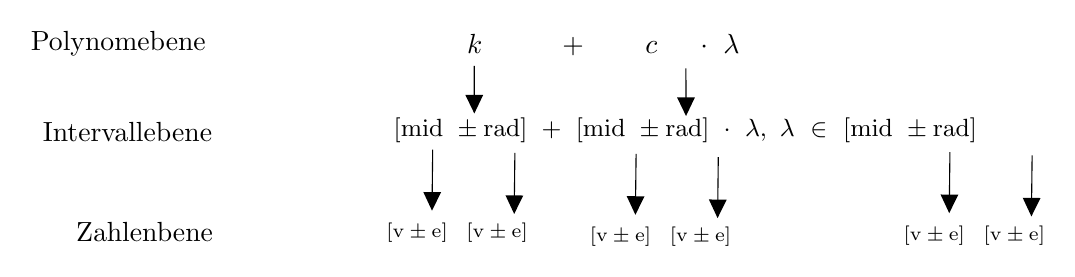
\begin{tikzpicture}[x=0.75pt,y=0.75pt,yscale=-1,xscale=1]
%uncomment if require: \path (0,300); %set diagram left start at 0, and has height of 300

%Straight Lines [id:da29898159624783616] 
\draw    (281.07,90.5) -- (280.77,116.88) ;
\draw [shift={(280.73,119.88)}, rotate = 270.65] [fill={rgb, 255:red, 0; green, 0; blue, 0 }  ][line width=0.08]  [draw opacity=0] (8.93,-4.29) -- (0,0) -- (8.93,4.29) -- cycle    ;
%Straight Lines [id:da1335093356184387] 
\draw    (320.67,92.1) -- (320.37,118.48) ;
\draw [shift={(320.33,121.48)}, rotate = 270.65] [fill={rgb, 255:red, 0; green, 0; blue, 0 }  ][line width=0.08]  [draw opacity=0] (8.93,-4.29) -- (0,0) -- (8.93,4.29) -- cycle    ;
%Straight Lines [id:da1340726243132735] 
\draw    (379.07,92.5) -- (378.77,118.88) ;
\draw [shift={(378.73,121.88)}, rotate = 270.65] [fill={rgb, 255:red, 0; green, 0; blue, 0 }  ][line width=0.08]  [draw opacity=0] (8.93,-4.29) -- (0,0) -- (8.93,4.29) -- cycle    ;
%Straight Lines [id:da9182990047680641] 
\draw    (418.67,94.1) -- (418.37,120.48) ;
\draw [shift={(418.33,123.48)}, rotate = 270.65] [fill={rgb, 255:red, 0; green, 0; blue, 0 }  ][line width=0.08]  [draw opacity=0] (8.93,-4.29) -- (0,0) -- (8.93,4.29) -- cycle    ;
%Straight Lines [id:da04610901450657834] 
\draw    (530.27,91.7) -- (529.97,118.08) ;
\draw [shift={(529.93,121.08)}, rotate = 270.65] [fill={rgb, 255:red, 0; green, 0; blue, 0 }  ][line width=0.08]  [draw opacity=0] (8.93,-4.29) -- (0,0) -- (8.93,4.29) -- cycle    ;
%Straight Lines [id:da7044032296577734] 
\draw    (569.87,93.3) -- (569.57,119.68) ;
\draw [shift={(569.53,122.68)}, rotate = 270.65] [fill={rgb, 255:red, 0; green, 0; blue, 0 }  ][line width=0.08]  [draw opacity=0] (8.93,-4.29) -- (0,0) -- (8.93,4.29) -- cycle    ;
%Straight Lines [id:da7628093943540135] 
\draw    (301.07,50.1) -- (301.12,70.08) ;
\draw [shift={(301.13,73.08)}, rotate = 269.84000000000003] [fill={rgb, 255:red, 0; green, 0; blue, 0 }  ][line width=0.08]  [draw opacity=0] (8.93,-4.29) -- (0,0) -- (8.93,4.29) -- cycle    ;
%Straight Lines [id:da9018979196177348] 
\draw    (403.07,51.3) -- (403.12,71.28) ;
\draw [shift={(403.13,74.28)}, rotate = 269.84000000000003] [fill={rgb, 255:red, 0; green, 0; blue, 0 }  ][line width=0.08]  [draw opacity=0] (8.93,-4.29) -- (0,0) -- (8.93,4.29) -- cycle    ;

% Text Node
\draw (86.2,32) node [anchor=north west][inner sep=0.75pt]   [align=left] {Polynomebene};
% Text Node
\draw (92,76) node [anchor=north west][inner sep=0.75pt]   [align=left] {Intervallebene};
% Text Node
\draw (108,124) node [anchor=north west][inner sep=0.75pt]   [align=left] {Zahlenbene};
% Text Node
\draw (296.4,33.8) node [anchor=north west][inner sep=0.75pt]    {$k\ \ \ \ \ \ \ \ +\ \ \ \ \ \  c\ \ \ \ \cdot \ \lambda $};
% Text Node
\draw (261,74) node [anchor=north west][inner sep=0.75pt]  [font=\small]  {$\left[\text{mid} \ \pm \text{rad}\right] \ +\ \left[\text{mid} \ \pm \text{rad}\right] \ \cdot \ \lambda ,\ \lambda \ \in \ \left[\text{mid} \ \pm \text{rad}\right]$};
% Text Node
\draw (257.5,124.6) node [anchor=north west][inner sep=0.75pt]  [font=\scriptsize]  {$\left[\text{v} \pm \text{e}\right] \ \ \left[\text{v} \pm \text{e}\right]$};
% Text Node
\draw (355.5,126.6) node [anchor=north west][inner sep=0.75pt]  [font=\scriptsize]  {$\left[\text{v} \pm \text{e}\right] \ \ \left[\text{v} \pm \text{e}\right]$};
% Text Node
\draw (506.7,125.8) node [anchor=north west][inner sep=0.75pt]  [font=\scriptsize]  {$\left[\text{v} \pm \text{e}\right] \ \ \left[\text{v} \pm \text{e}\right]$};


\end{tikzpicture}
  
 \caption{Ebenen der Polynomdarstellung mit REALs}
 \label{fig:levels}
 \end{center}
\end{figure}


\section{Intervallarithmetik}

Arithmetik auf Taylormodellen zu betreiben bedeutet auf der untersten Ebene, mit Intervallen zu rechnen. Um diese wiederum als Zahlentyp zu verwenden, müssen die Operationen angepasst werden \cite{moore1979}.

\paragraph{Grundrechenarten}
\begin{itemize}
    \item[] $[x_1, x_2] + [y_1, y_2] = [x_1 + y_1, x_2 + y_2]$
    \item[] $[x_1, x_2] - [y_1, y_2] = [x_1 - y_2, x_2 - y_1]$
    \item[] $[x_1, x_2] \cdot [y_1, y_2] = [min(x_1 y_1, x_1 y_2, x_2 y_1, x_2 y_2), max(x_1 y_1, x_1 y_2, x_2 y_1, x_2 y_2)]$
    \item[] $[x_1, x_2] / [y_1, y_2] = [min(x_1 / y_1, x_1 / y_2, x_2 / y_1, x_2 / y_2),$\\ $max(x_1 /y_1, x_1 /y_2, x_2 /y_1, x_2 /y_2)]$
\end{itemize}
\paragraph{Potenzfunktion}\label{par:potenzfunktion}
Die Potenzfunktion unterscheidet zwischen geradem und ungeradem Exponenten.
$$[x_1, x_2]^n =
 \begin{cases}
    [x_1^n, x_2^n] & falls\ x_1 > 0\ oder\ n\ ungerade; \\
    [x_2^n, x_1^n] & falls\ x_2 < 0\ und\ n\ gerade, \\
    [0, max(x_1^n, x_2^n)] & falls\ 0\in [x_1, x_2] \ und\ n\ gerade;
 \end{cases}$$

\paragraph{Kehrwert}
Der Kehrwert eines Intervalls kann nur bestimmt werden, wenn es nicht die 0 enthält:
$$
1/[x_1, x_2] = [1/x_2, 1/x_1]
$$
Wenn $x_1 \leq 0\leq x_2$, bedeutet das, dass für ein $x\in [x_1, x_2]$, $\frac{1}{x} \geq \frac{1}{x_2}$ oder $\frac{1}{x} \leq \frac{1}{x_1}$ gelten muss und das Intervall damit unbegrenzt ist.


Die im Basisprogramm \verb+tangentspace+ vorhandene Implementierung wurde erweitert, um Punktintervalle gesondert zu behandeln und die nun auf reellen Zahlen basierenden Intervalldefinitionen zu verwenden. Dies hat zur Folge, dass die Mehrwertigkeit der Vorzeichenfunktion berücksichtigt werden muss. Tritt der Fall der Unsicherheit ein, so muss mit einer Überschätzung gerechnet werden, die in jedem Fall korrekt ist.




%% ==============================
\section{Polynommultiplikation}
%% ==============================
\label{ch:Implementierung:sec:Abschnitt1}

In einer linearen Implementierung der Taylormodelle wird bei der Multiplikation immer eines der Fehlersymbole gesweept, sodass die Länge eines Polynoms nicht über die Dimension hinausgeht und somit der Schwerpunkt bei der Intervallarithmetik liegt. Lässt man allerdings höhere Ordnungen zu, werden auch die Polynome länger und ein weiteres Problem tritt auf. Um die oben (\ref{def:order}) definierte Ordnung $\prec$ auf dem Polynom $p = p_1 \cdot p_2$ zu erhalten, müssen die $n\cdot m$ Monome ($n := \#p_1, m := \#p_2$), die bei der Multiplikation entstehen, sortiert werden. Werden diese sequentiell zu $p$ hinzugefügt bedeutet das 2 Vergleiche, dann 3, dann 4, und so weiter, bis hin zu $nm$ Vergleichen:
$$ 2 + 3 + 4 + 5 + ... + nm = \frac{nm \cdot (nm + 1)}{2} - 1$$
So ergibt sich für die naive Multiplikation eine quadratische Laufzeit in $O$-Notation von $O(nm + (nm)^2)$
\par
Für effizientere Polynommultiplikation existieren verschiedene Algorithmen. Viele der schnellen bekannten Algorithmen basieren  auf der Schnellen-Fourier-Transformation, wobei die Polynome in Stützvektoren und wieder zurück umgewandelt werden. Da es sich bei den Koeffizienten den Monome um Intervalle mit möglicherweise unendlichen Schranken handelt, ist das Rückführen eines Stützvektors nicht immer ohne Weiteres möglich. \par
Ein weiterer Ansatz besteht darin, die Anzahl der benötigten Monomvergleiche zu reduzieren, wenn die Monome einsortiert werden müssen. Betrachtet man die Summe dreier Polynome $p_1 + p_2 + p_3$ mit $\#p_1 >> \#p_2 = \#p_3 = 1$, benötigt das Aufsummieren von links nach rechts $2\#p_1 + 1$ Vergleiche, da mit dem oben verwendeten Additionsverfahren zweifach in $p_1$ eingefügt wird. Summiert man jedoch von rechts nach links so werden lediglich $\#p_1 + 2$ Vergleiche benötigt. Nach dieser Idee kann die Anzahl der Monomvergleiche reduziert werden, indem zunächst Polynome gleicher Länge miteinander addiert werden. Mit Geobuckets, von Yan (\cite{geobuckets}) eingeführt und Monagan und Pearce (\cite{geobucketsmulti}) für die Multiplikation angepasst, werden die Zwischenergebnisse der Polynommultiplikation in geometrisch wachsenden 'Buckets' gespeichert. Hat ein Bucket seine Kapazität erreicht, wird das Polynom zum nächst größeren Bucket hinzuaddiert. Der Unterschied zum Originalalgorithmus besteht darin, dass die Größe der hinzukommenden Polynome bereits bekannt ist und die Bucketkapazität dementsprechend angepasst werden kann. Algorithmus \ref{algo:mult} zeigt die in \verb+hotm+ implementierte Version der Geobucketmultiplikation. Durch den Teile und Herrsche Ansatz, kann die Multiplikation mit Geobuckets in $O(nm \log nm)$ durchgeführt werden.  \par


Wird wie in \cite{geobuckets} eine Ordnung $\succ$ auf den Monomen definiert, können die Polynome sortiert werden.
\begin{itemize}
    \label{def:order}
    \item $\lambda_1 \succ \lambda_2 \succ...\succ \lambda_k $
    \item $\lambda_n^i \lambda_m^j \succ \lambda_n^{i'} \lambda_m^{j'} $ für $n > m$, falls
    \begin{itemize}
        \item[] $ i > i'$, oder
        \item[] $ i = i'$ und $ j > j'$
    \end{itemize}
\end{itemize}
Diese Ordnung ist partiell, da gleiche Monome, beziehungsweise Monome mit gleichen Fehlersymbolen nicht vergleichbar sind. Tritt dieser Fall während der Addition zweier Polynome auf, bedeutet das, dass die Koeffizienten beider Monome addiert werden und das so entstandene Monom in das Polynom aufgenommen wird.
Haben die verglichenen Monome die selbe Anzahl an Variablen, entscheidet die Größe des Exponenten des Fehlersymbols mit dem kleinsten Index. Algorithmus \ref{algo:maxes} implementiert den Vergleich zweier Monome, beziehungsweise derer Variablen.

\begin{figure}[ht]
    \centering
    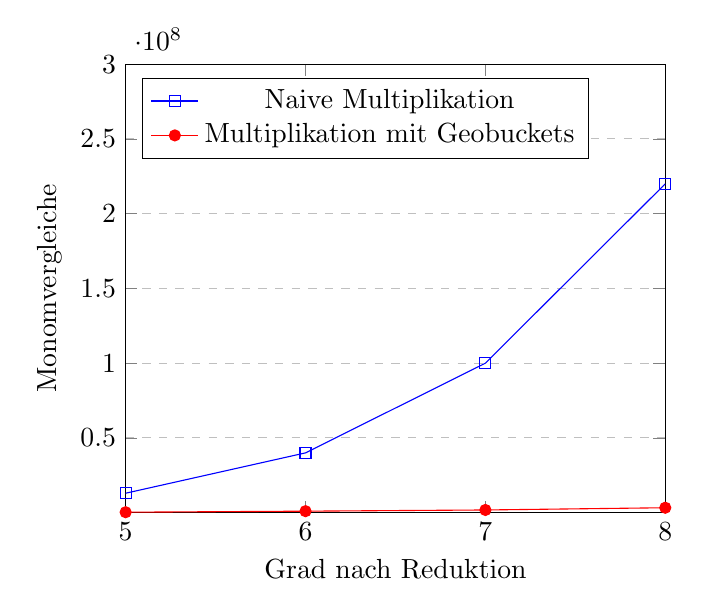
\begin{tikzpicture}
    \begin{axis}[
        xlabel={Grad nach Reduktion},
        ylabel={Monomvergleiche},
        xmin=5, xmax=8,
        ymin=100000, ymax=300000000,
        xtick={5,6,7,8},
        legend pos=north west,
        ymajorgrids=true,
        grid style=dashed,
    ]
    \addplot[
        color=blue,
        mark=square
        ]
        coordinates {
        (5, 13000000)(6, 40000000 )(7, 100000000)(8, 220000000)
        };
        \addlegendentry{Naive Multiplikation}
        
    \addplot[
        color=red,
        mark=*
        ]
        coordinates {
        (5, 300000)(6, 1000000 )(7, 1800000)(8, 3300000)
        };
        \addlegendentry{Multiplikation mit Geobuckets}
    
    \end{axis}
    \end{tikzpicture}
    \caption{Naive Multiplikation gegen Multiplikation mit Geobuckets}
    \label{fig:my_label}
\end{figure}



\newpage
%% ==============================
\section{Taylormodelle}
Taylormodelle bestehen in \verb+hotm+ aus einer List von nach der Ordnunng $\succ$ (siehe \ref{def:order}) sortierten Monomen. Für die Supportintervalle der Fehlersymbole wird eine statische Liste (\verb+static std::list+), für die Grenzwerte der Housekeeping-Methoden und den Index neuer Fehlersymbole jeweils statische Variablen angelegt.
\subsection{Housekeeping-Methoden}
Die Housekeeping-Methoden Splitting und Sweeping werden in \cite{DBLP:conf/macis/BrausseKM15} beschrieben und dienen der Kontrolle der Intervallkoeffizieten und deren Wachstum. Wann die Methoden angewandt werden, wird durch die manuell justierbaren Parameter \verb+MACRO_THRESHOLD+ für Splitting und \verb+MICRO_THRESHOLD+ für Cleaning festgelegt. Da für diese beiden Methoden Vergleiche reeller Zahlen nötig sind, um das Überschreiten eines Grenzwertes zu bestimmnen, werden die Zahlen mit Funktionen der \verb+iRRAM+ in rationale Approximationen zerlegt.

\paragraph{Cleaning}
Wie oben beschrieben, ergibt die Verwendung der \verb+iRRAM-REAL+s als Intervallgrenzen zweistufige Intervalle mit der Zahlen- und Intervallebene (siehe Abbildung \ref{fig:levels}). Mit fortlaufenden Rechnungen wächst die Breite der Intervalle auf Zahlenebene kontinuierlich und kann ohne weitere Methoden nur durch ein Erhöhen der verwendeten Präzision wieder verringer werden, beziehungsweise durch eine Iteration der \verb+iRRAM+. \textit{Cleaning} verlagert den Rechenfehler der Zahlenebene auf die Intervallebene und macht ihn damit auch für andere Housekeeping-Methoden sichtbar. Das Intervall $I=[m \pm r]$ mit $m=[c_m \pm \varepsilon_m]$ und $r = [c_r \pm \varepsilon_r]$ wird um $\varepsilon_m$ und $\varepsilon_r$ vergrößert, sodass das $I$ zwar wächst, jedoch dessen Endpunkte exakt sind:
\begin{align*}[[c_m \pm \varepsilon_m] \pm [c_r \pm \varepsilon_r]] &\rightsquigarrow [[c_m \pm 0] \pm [c_r + \varepsilon_m +\varepsilon_r  \pm 0]] \\
&= [\underbrace{c_m'}_{c_m + \varepsilon_m +\varepsilon_r} \pm c_r ]\end{align*}
    
    

\paragraph{Splitting}
Durch Cleaning, Sweeping oder eine Initialisierung der Taylormodelle mit einer gewissen Breite wachsen die Radii der Koeffizienten im Laufe einer Berechnung auch auf Intervallebene. Um die Überschätzung, die durch Intervallarithmetik entsteht zu kontrollieren, kann durch \textit{Splitting} ein Monom in zwei Monome mit Punktintervallen als Koeffizienten und einem neuen Fehlersymbol aufgeteilt werden:
\begin{align*}
[\tilde{c}_n \pm \varepsilon_n]\ \rightarrow [\tilde{c}_n \pm 0] + [\varepsilon_n \pm 0]\cdot  \lambda_n \hspace{0.5cm}, \lambda_n \in [0 \pm 1]
\end{align*}
Dadurch erhöht sich der Grad des Polynoms, jedoch verringert sich die Überschätzung durch Intervallarithmetik. Eine Alternative das Splitting zu realisieren ist, den Fehler statt wie in \cite{DBLP:conf/macis/BrausseKM15} im Koeffizienten des neuen Monoms, im neuen Fehlersymbol zu kodieren:
\begin{align*}
 [\tilde{c}_n \pm \varepsilon_n]\ \rightsquigarrow [\tilde{c}_n \pm 0] + [1 \pm 0]\cdot  \lambda_n \hspace{0.5cm}, \lambda_n \in [0 \pm \varepsilon_n]
\end{align*}
Dies hat den Vorteil, dass die Größe der Fehlersymbole beim Sweeping berücksichtigt werden kann.

\paragraph{Sweeping}
Cleaning und Splitting sorgen dafür, dass die Intervallbreite der Koeffizienten klein bleibt, jedoch erhöht sich der Grad der Polynome, was zum Beispiel bei der Multiplikation von Taylormodellen zu Ineffizienz durch die exponentiell wachsende Anzahl an Monomen führt. Um diesem Effekt entgegenzuwirken, kann mit \textit{Sweeping} ein Fehlersymbol durch sein Supportintervall ersetzt werden:
\begin{align*}
 c_n \lambda_i^k \rightsquigarrow c_n s_i \lambda_i^{k-1}
\end{align*}
Hierbei ist zu beachten, dass das $n$-fache Sweepen eines Fehlersymbols, welches die 0 enthält, mit $n$ gerade eine geringere Breite in den Koeffizienten einführt, als $n$ ungerade (siehe oben \ref{par:potenzfunktion}). Daraus ergeben sich zwei Sweeping-\textit{Strategien}.

\subparagraph{square\_only}
Die Sweeping-Strategie \verb+square_only+ beschränkt das Sweeping auf gerade Potenzen. So wird die angestrebte Reduktion des Grades eines Monoms nur erreicht, wenn alle Variablen einen geraden Exponenten haben.


\subparagraph{square\_first}
Mit \verb+square_first+ wird der angestrebte Grad erreicht, indem zunächst möglichst viele Fehlersymbole gerade gesweept werden. Falls dadurch jedoch nicht die gesamte Reduktion möglich ist, wird der Rest ungerade gesweept.

Der Aufruf der Methode erhält in \verb+hotm+ drei Parameter; das zu reduziere Taylormodell, den Grad, auf das Taylormodell durch Sweeping reduziert werden soll und die Strategie:

 \begin{lstlisting}[language=C++]
tmsimple x;
x = sweep_to(x, 2, SQUARE_ONLY);
\end{lstlisting}













%%% Local Variables: 
%%% mode: latex
%%% TeX-master: "thesis"
%%% End: 
    % Implementierung
%% eval.tex
%% $Id: eval.tex 61 2012-05-03 13:58:03Z bless $

\chapter{Evaluation}
\label{ch:Evaluierung}
%% ==============================

Werden die Initialwerte für Iterationen der H\e non-Abbildung $(x_0, y_0)$ als Taylormodelle mit Itervallen definiert, kann eine Fläche beschrieben werden, die durch die Abbildung gespiegelt, gedehnt und verzerrt wird. Liegt diese für $a=1.4$ und $b=0.3$ komplett innerhalb der Fangzone $R$, so wird jeder Punkt in der Fläche wiederum nach $R$ abgebildet. 

\Abbildungps{tbh}{.7}{img/6iter.pdf}{fig:escape}{H\e non-Abbildung: Mehrere Iterationen mit großen Initialwerten}{Iterationen der H\e non-Abbildung ausgehend von einem größeren Rechteck}

Eine Abbildung der Fläche im Ganzen führt jedoch zu einer Überschätzung, die in jeder Iteration zunimmt, da nun mit Intervallen statt mit Punkten gerechnet wird. Abbildung \ref{fig:escape} zeigt pro Graph eine Iteration mit 
\begin{align*}
x_0 = 0 + 1 \cdot \lambda_1 & \hspace{0.5cm} (\lambda_1 \in [0 \pm 0.4]) \\
 y_0 = 0 + 1 \cdot \lambda_2 & \hspace{0.5cm} (\lambda_2 \in [0 \pm 0.1])
\end{align*}
und der Fangzone als schwarzes Tetragon. Es ist erkennbar, dass das Rechteck nach wenigen Iterationen die Fangzone verlässt und einige Itervalle ein starkes Rauschen verursachen. Abbildung \ref{fig:7iter} zeigt  Iterationen mit kleineren initialen Intervallen, wodurch die Überschätzung erst zu einem späteren Zeitpunkt zu groß wird. Um dem Wachstum der Intervalle entgegenzuwirken und die Berechnung der H\e non-Abbildung auch für solche Flächem mit höheren Iterationszahlen zu ermöglichen, könnten die Taylormodelle in Partitionen aufgeteilt werden.  Die kleinste Partitionierung wäre die Aufteilung der Fläche in unendlich viele Punkte, was nicht praktikabel wäre, allerdings hohe Iterationszahlen ermögliche, wie in Abbildung \ref{fig:strangeattractor} zu sehen ist. Das andere Extrem stellen große Itervalle, beziehungsweise keine Partitionierung dar, was im Vergleich nur einen Bruchteil des Rechenaufwandes bedeutet, jedoch schnell zu starker Überschätzung führt.

In diesem Kapitel wird untersucht, wie sich die \verb+HOTM+ bei verschiedenen Intervallgrößen verhalten und welche Konfiguration der Parameter für die Housekeeping-Methoden und den Taylormodellen selbst zu einer möglichst kleinen Überschätzng führt.
Der Housekeeping-Vorgang der in jeder Iteration bei den Taylormodellen angwandt wird besteht aus vier Schritten:
 \begin{enumerate}
  \item \textbf{(Sweeping)} Reduktion des Taylormodells bis zum angegebenen Grad, je nach Strategie
  \item \textbf{(Sweeping überschüssiger Fehlersymbole)} Entfernen aller Fehlersymbole bis auf die $n$-größten (abhängig von deren Support-Space)
  \item \textbf{(Cleaning)} Verlagern der durch die Schritte 1 und 2 entstandenen Rechenfehler auf der Ebene der \verb+iRRAM-REAL+s auf die Radii der Intervalle
  \item \textbf{(Splitting)} Einführen neuer Fehlersymbole für Monome, deren Koeffizienten durch die Schritte 1-3 zu stark gewachsen sind.
 \end{enumerate}

% Um die Fragestellung, wie die H\e non-Abbildung mit Taylormodellen am besten berechnet werden kann zu erörtern, wird das Problem in drei Sektionen unterteilt:
% 
% \begin{enumerate}
%  \item Wie klein müssen die Taylormodelle sein, damit längere Berechnungen möglich sind?
%  \item Wie verhalten sich die verschiedenen Partitionsgrößen bei unterschiedlichen Konfigurationen der Taylormodelle?
%  \item Welche Partition ist für eine gegebene Anzahl an Iterationen nötig?
% \end{enumerate}
% 



Die Implementierung nichtlinearer Taylormodelle ergibt eine Vielzahl von Konfigurationsmöglichkeiten und damit einen großen Suchraum nach der optimalen Einstellung:
\begin{itemize}
 \item Grenzwert für Cleaning $\delta_c$, Splitting $\delta_s$
 \item Grad der Reduktion durch Sweeping
 \item Anzahl der zu erhaltenden Fehlersymbole
 \item Strategie beim Sweeping
 \item Heuristik für die Reihenfolge, in der Fehlersymbole gesweept werden
 \item Vorgehen beim Splitting
 \item Definition des initialen Taylormodells
\end{itemize}
Diese Konfigurationen können in \verb+HOTM+ als JSON-Datei mit Hilfe einer JSON-Bibliothek\footnote{\url{https://github.com/nlohmann/json} (Stand Dezember 2020)} eingelesen und verarbeitet werden, um wiederholte Durchläufe mit leicht veränderten Parametern oder Batch-Runs zu vereinfachen. Listing \ref{list:config} zeigt ein Beispiel einer Konfigurationsdatei, mit der versuchsweise 1000 Iterationen der H\e non-Abbildung berechnet werden sollen. 



\section{Housekeeping-Grenzwerte}
Der Grenzwert einer Housekeeping-Methode gibt an ab welchem Wert die jeweilige Methode angewandt wird. Bei einem intervall in \verb+HOTM+ $I=[m \pm r]$ mit $m = [c_m \pm \varepsilon_m]$ und $r = [c_r \pm \varepsilon_r]$ als \verb+iRRAM-REAL+s wird
\begin{itemize}
 \item Cleaning angewandt, wenn $\varepsilon_m < \delta_c$ oder $\varepsilon_r < \delta_c$ gilt und
 \item Splitting angewandt, wenn $c_m < \delta_s$ oder $c_m < \delta_s$ gilt.
\end{itemize}
Um diese Werte zu untersuchen, wurde betrachtet, wie sich die Größe des Rechtecks, welches durch die Intervalle $x$ und $y$ aufgespannt wird, abhängig von den Grenzwerten $\delta_c$ und $\delta_s$ entwickelt, beziehungsweise, wieviele Iterationen der H\e non-Abbildung bei einer festen Genauigkeit der \verb+iRRAM-REAL+s möglich sind, bis das Rechteck eine Fläche von $>2^{-5}$ erreicht hat\footnote{Ab einer Fläche von zirka $2^-{5}$ ist die Überschätzung der Intervalle zu groß und wächst innerhalb weniger Iterationen ($< 10$) gegen $\infty$.}.


\begin{table}[tbh]
\centering
\begin{tabular}{ll}
\begin{tabular}{|l|l||c|c|}
\hline \multicolumn{3}{|c|}{\begin{tabular}[c]{@{}c@{}}1000 Bits Präzision \\$x=[0 \pm 2^{-1000}], y=[0 \pm 2^{-1000}]$\\ \end{tabular}}                                                                                                                                                                                                                              \\ \hline
\multicolumn{1}{|c|}{\begin{tabular}[c]{@{}c@{}}$\delta_c$\\($2^{-\delta_c}$)\end{tabular}} & \multicolumn{1}{c||}{\begin{tabular}[c]{@{}c@{}}$\delta_s $\\($2^{-\delta_s}$)\end{tabular}} & \begin{tabular}[c|]{@{}c@{}}Iterationen \end{tabular}   \\ 
\hline
- & - & 451  \\
10   & 10       & 162     \\
10   & 5       & 160      \\
100  & 100      & 273     \\
100  & 50      & 258      \\
500  & 500      & 794     \\
500  & 250      & 746      \\
1000 & 1000     &  1432 \\                                   
1000 & 500    & 1317 \\                                    

\hline 
\end{tabular}
&
\begin{tabular}{|l|l||c|c|}
\hline \multicolumn{3}{|c|}{\begin{tabular}[c]{@{}c@{}}10000 Bits Präzision \\$x=[0 \pm 2^{-10000}], y=[0 \pm 2^{-10000}]$\\ \end{tabular}}                                                                                                                                                                                                                              \\ \hline
\multicolumn{1}{|c|}{\begin{tabular}[c]{@{}c@{}}$\delta_c$\\($2^{-\delta_c}$)\end{tabular}} & \multicolumn{1}{c||}{\begin{tabular}[c]{@{}c@{}}$\delta_s $\\($2^{-\delta_s}$)\end{tabular}} & \begin{tabular}[c|]{@{}c@{}}Iterationen \end{tabular}   \\ 
\hline
- & - & 4360  \\
100  & 100      & 1463     \\
100  & 50      & 1450      \\
1000 & 1000     &  2641 \\                                   
1000 & 500    & 2530 \\           
5000  & 5000      & 7849     \\
5000  & 2500      & 7289      \\
10000 & 10000     &  14455 \\                                   
10000 & 5000    & 13401 \\                                    
\hline 
\end{tabular}

\end{tabular}
\caption[Experimentelle Ergebnisse zu Grenzwerten]{Berechnung der Fläche des Rechtecks mit verschiedenen Grenzwerten für Cleaning $\delta_c$ und Splitting $\delta_s$ und festgelegter Präzision.}
\label{tab:housekeeping}
\end{table}

Tabelle \ref{tab:housekeeping} zeigt experimentelle Ergebnisse für $x_0 = 0 + 1 \cdot \lambda_1 $ und $y_0 = 0 + 1 \cdot \lambda_2$ mit $\lambda_1, \lambda_2 \in [0 \pm \varepsilon]$. Sowohl für 1000, als auch für 10000 Bits Genauigkeit reagiert das Ergebnis sehr sensibel auf die Grenzwerte der Housekeeping-Methoden. Falsch gewählte Werte vergrößern sogar die entstandene Überschätzung im Vergleich zu einer Berechnung ohne Cleaning und Splitting, jeweils in Zeile 1 der Tabellen zu sehen. Werden die Grenzwerte durch die \verb+iRRAM+-Präzision bestimmt, so bleibt der Fehler am längsten klein und die höchste Iterationszahl ist möglich.

\Abbildungps{tbh}{.6}{img/housesteps.png}{fig:housesteps}{Experimentelle Ergebnisse zu Grenzwerten}{Iterationszahl der H\e non-Abbildung mit fester Genauigkeit von 1000 Bits.}

Wie in Abbildung \ref{fig:housesteps} zu sehen ist, hat eine Definition der Grenzwerte unter die zugrunde liegende Genauigkeit keinen Effekt mehr auf die Performanz der Berechnung und die Iterationszahl erhöht sich nicht weiter. Der Grund hierfür ist, dass die Anwendung von Methoden der \verb+iRRAM+ auf die sehr kleinen Intervalle zu einer Skalierung auf die gegebene Genauigkeit führt.

\section{Sweeping}
 Für eine Sweeping-Konfiguration kommen drei einander beeinflussende Parameter in Betracht: die Sweeping-Strategie, die Gradreduktion und die Anzahl der zu erhaltenen Fehlersymbole. 
 Abbildung \ref{fig:sweeping} zeigt die Performanz der Berechnung der H\e non-Abbildung, gemessen an der erreichten Iterationszahl mit statischer Präzision in verschiedenen Fällen. Wie zuvor ist die Berechnung beendet, sobald die Fläche des Rechtecks einen Schwellenwert überschreitet. Zu sehen ist, bei welcher Kombination von Parametern für Sweeping (Schritt 1) und Sweping überschüssiger Fehlersymbole (Schritt 2) die Überschätzung am langsamsten wächst und somit die meisten Iterationen errechnet werden können. Die Zeiteffizienz ist in diesem Falle kein Faktor. Es ist zu erkennen, dass sich die Graphen innerhalb derselben Sweeping-Strategie kaum unterscheiden. Eine Verzehnfachung des Exponenten in der Breite der Intervalle und der Bits für die Präzision verzehnfacht auch die erreichte Iterationszahl. Die besten Ergebnisse werden beim Beschränken auf \textbf{square\_only} (quadratisches Sweeping) für $n=3$ und Sweeping zum Grade 0; bei \textbf{square\_first} für $n=1$, $n=4$ und Sweeping zum Grade 3 erreicht. Insgesamt wird jedoch mit \textbf{square\_only} zum Grade 0, also einem Sweeping bis zu einem Taylormodell, dessen Monome Variablen mit höchstens Grad 1 haben, die höchste Iterationszahl erzielt:

$$ c \cdot \lambda_1^3 \lambda_2^2 \lambda_3^1 \lambda_4^3  \underset{square\_only}{\overset{sweep\ to\ 0}{\rightsquigarrow}} c' \cdot \lambda_1^1 \lambda_2^0 \lambda_3^1 \lambda_4^1$$



\begin{figure}[tbh]
\centering
\begin{subfigure}{.5\textwidth}
  \centering
  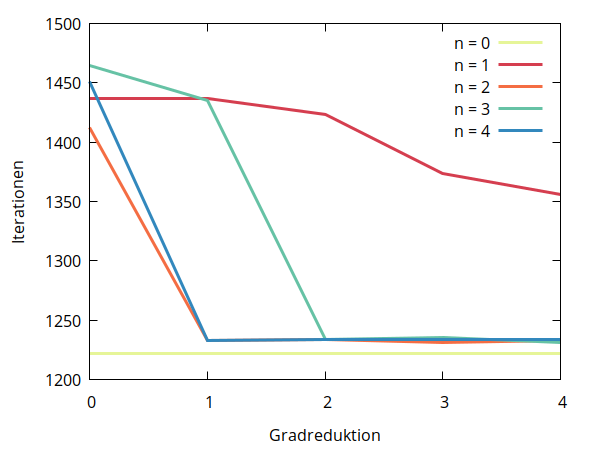
\includegraphics[width=\linewidth]{img/sweeping_only.png}  
  \caption{Sweeping beschränkt \textbf{square\_only}}
  \label{fig:sub1}
\end{subfigure}%
\begin{subfigure}{.5\textwidth}
  \centering
  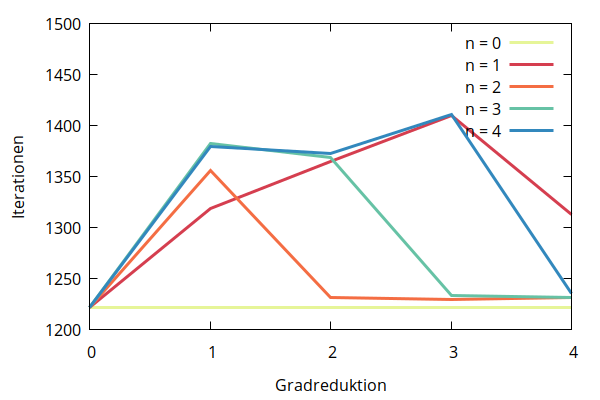
\includegraphics[width=\linewidth]{img/sweeping_first.png}
 \caption{Sweeping beschränkt \textbf{square\_first}}
  \label{fig:sub2}
\end{subfigure}

\begin{subfigure}{.5\textwidth}
  \centering
  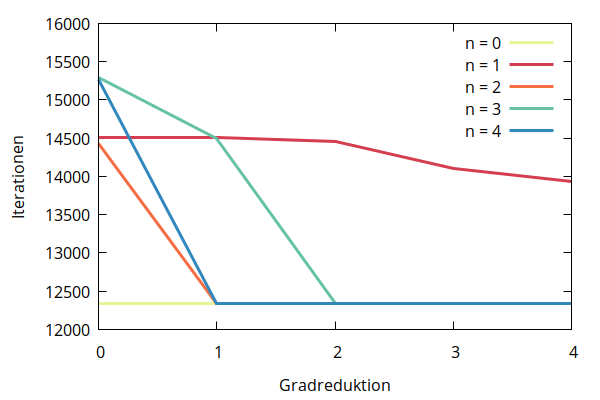
\includegraphics[width=\linewidth]{img/sweeping_only10k.png}
  \caption{Sweeping beschränkt \textbf{square\_only}}  
  \label{fig:sub1}
\end{subfigure}%
\begin{subfigure}{.5\textwidth}
  \centering
  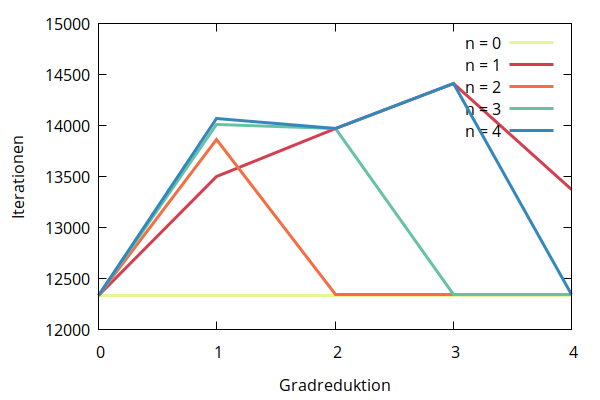
\includegraphics[width=\linewidth]{img/sweeping_first10k.png}
 \caption{Sweeping beschränkt \textbf{square\_first}}
  \label{fig:sub2}
\end{subfigure}
\caption[Sweeping mit verschiedenen Graden]{Anzahl an Iterationen mit Erhalt der n größten Fehlersymbole. (a) (b): 1000 Bits Präzision , $x_0 = y_0 = [0 \pm 2^{1000}]$.
 (c)(d): 10000 Bits Präzision , $x_0 = y_0 = [0 \pm 2^{10000}]$
}
\label{fig:sweeping}
\end{figure}

Im Vergleich mit rein linearen Taylormodellen zeigt sich eine Verbesserung (siehe Abbildung \ref{fig:extra}). Der Unterschied besteht darin, dass die nichtlinearen Taylormodelle während der Berechnung und besonders während der Multiplikation Punktintervalle erhalten können und sich stattdessen der Grad und die Länge des Polynoms erhöht. Nach jeder Iteration werden dann verschiedene Monome durch Gradreduktion vereint, wobei die Intervalle breiter werden. Im nächten Schritt wird der Grad dann durch Splitting auf den Monomen um maximal 1 erhöht und es liegen wieder Punktintervalle vor. Für lineare Taylormodelle steht lediglich das Splitting für den Kernel zur Verfügung, da sonst nichtlineare Polynome entstünden. Des Weiteren wird hier bereits während der Multiplikation gesweept und Punktintervalle werden zu regulären Intervallen. Die Performanz des Sweepings \textbf{square\_only} zum Grade 0 verbessert sich im Schnitt mit einer wachsenden Zahl der zu erhaltenen Fehlersymbole, wie in Abbildung \ref{fig:extra} zu sehen ist. Jedes Fehlersymbol erhöht die Menge an erhaltener Abhängigkeitsinformation und sorgt dafür, dass ein Taylormodell dessen Ränder besser beschreiben kann. Allerdings stellt die Praktikabilität dieser Herangehensweise ein Problem dar, da so sehr große Polynome entstehen, die während einer Iteration der H\e non-Abbildung exponentiell in ihrer Länge wachsen.
 

 \Abbildungps{tbh}{.7}{img/extra.png}{fig:extra}{Experimentelle Ergebnisse zu erhaltenen Fehlersymbolen}{Gegenüberstellung von $x_0 = y_0 = [0 \pm 2^{10000}]$ als lineare Taylormodelle und nichtlineare Taylormodelle mit quadratischem Sweeping zum Grade 0. Jeweils bleiben verschiedene Anzahlen von Fehlersymbolen pro Iteration erhalten. Gemessen wird die Iterationszahl der H\e non-Abbildung mit fester Genauigkeit von 10000 Bits, bis $|x_n|\cdot|y_n|$ einen Grenzwert von $2^{-6}$ überschreitet. }

 Dieser Effekt ist in Tabelle \ref{tab:time} verdeutlicht. Eine Erhöhung der Anzahl der erhaltenen Fehlersymbole hat einen drastischen Einfluss auf die durchschnittliche Dauer einer Iteration in $ms$, bis das Programm bei größeren Werten quasi nicht mehr lauffähig ist ($>100ms$ pro Iteration). Betrachtet man nun das Verhältnis zwischen der Verbesserung der Performanz (Abbildung \ref{fig:extra}) und der Verschlechterung der Laufzeit (Tabelle \ref{tab:time}), so bildet das Setzen der erhaltenen Fehlersymbole auf 3 mit einem Zielgrade von 0 bei der Beschränkung auf quadratisches Sweeping einen guten Trade-off, weshalb diese Konfiguration als Voreinstellung für Sweeping in der Implementierung (Kapiter \ref{ch:umsetung}) vorgesehen ist.
 
  
 \begin{table}[tbh]
\centering
\begin{tabular}{|c||c|c|c|c|c|}
\hline
&\multicolumn{5}{c|}{Erhaltene Fehlersymbole pro Iteration} \\
\hline
Gradreduktion & 0 & 1 &2& 3 & 4\\
\hline
0& 0.166& 0.603&    2.097&   4.358&    13.354\\
1& 0.166& 0.939&   2.358&  7.470&   >100\\
2& 0.166& 1.645&     5.750&   20.339 &    >100\\
3& 0.166& 2.284&     2.977&   74.172&    >100\\
4&0.166& 2.658&    3.622&   >100    &   >100\\
\hline 
&\multicolumn{5}{c|}{$ms$ pro Iteration} \\
\hline
\end{tabular}

\caption[Experimentelle Ergebnisse zu erhaltenen Fehlersymbolen]{Durchschnittliche Dauer einer Iteration der H\e non-Abbildung in $ms$ mit Taylormodelle der Größe $[0\pm 2^{-10000}]$ bei festgelegter Präzision von 10000 Bits und 1000 Iterationen.}
\label{tab:time}
\end{table}
 
 
 \section{Cleaning}
 Durch die mehrstufige Intervallstruktur in den Koeffizienten der Polynome ist es mit Cleaning möglich, den Rechenfehler, beziehungsweise die Intervallbreite der Intervallgrenzen auf einer höheren Abstraktionsebene zu verwalten. Wie in Paragraph \ref{par:cleaning} beschrieben, wird das Intervall um die Intervallbreite des Mittelpunktes und des Radius' erweitert und schließt es somit komplett ein. Dies hat darüber hinaus den Effekt, dass sämtlicher entstandene Rechenfehler durch Anwendung von Splitting reduziert werden kann. 
 
   \Abbildungps{tbh}{.7}{img/clean.png}{fig:clean}{Experimentelle Ergebnisse zum Effekt des Cleaning}{Iterationszahl der H\e non-Abbildung mit festem Radius der intialen Taylormodelle $x_0 = y_0 = [0 \pm 2^{-1000}]$ mit wachsender Präzision, um den Effekt des Cleanings beschreiben.}
 
 Abbildung \ref{fig:clean} zeigt die Auswirkung der Anwendung von Cleaning bei initialen Taylormodellen $x_0, y_0$ der Breite $2^{-1000}$ mit wachsender Genauigkeit. Cleaning sorgt für ein langsameres Wachstum des Rechtecks $|x_n|\cdot|y_n|$ nach $n$ Iterationen im Vergleich zur Berechnung ohne Cleaning. Bei einer höheren Anzahl der erhaltenen Fehlersymbole pro Iteration wird der Effekt noch deutlicher, da nun mit deutlich längeren Polynomen gerechnet und dementsprechend mehr arithmetische Operationen auf den Koeffizienten angewandt werden. So bleibt zwar mehr Information über Form der Taylormodelle erhalten, jedoch dominiert die Überschätzung auf der Zahlenebene das Ergebnis beim Verzicht auf Cleaning, während sich die Performanz im anderen Fall leicht verbessert.
 

 
 
 \section{Splitting}
 Durch Splitting wird ein Monom mit Intervallkoeffizienten in zwei Monome mit einem neuen, noch nicht verwendeten Fehlersymbol und Punktintervallkoeffizienten aufgeteilt. Für diese Housekeeping-Methode wurden zwei Möglichkeiten betrachtet. Zum Einen die in \cite{DBLP:conf/macis/BrausseKM15} verwendete Definition des neuen Fehlersymbols als Einheitsintervall:
 
\begin{align}
\label{int:unit}
 [c \pm \varepsilon]  \underset{split}{\rightsquigarrow} [c] + [\varepsilon] \cdot \lambda_{new}, \lambda_{new} \in [0 \pm 1]
\end{align}

Zum Anderen die Umlagerung des Radius $\varepsilon$ in das neue Fehlersymbol:

\begin{align}
\label{int:nunit}
 [c \pm \varepsilon]  \underset{split}{\rightsquigarrow} [c] + [1] \cdot \lambda_{new}, \lambda_{new} \in [0 \pm \varepsilon]
\end{align}
 
Beim Sweeping hat sich gezeigt, dass die Überschätzung des Taylormodells bei einer Priorisierung kleinerer Fehlersymbole, beziehungsweise durch Erhalt von Fehlersymbolen mit größerem Support-Space, langsamer wächst. In einer linearen Implementierung der Taylormodelle mit Variante \ref{int:unit} wird eine solche Ordnung durch einen Vergleich der Koeffizienten hergestellt, da jedes Monom maximal ein Fehlersymbol enthalten kann. Ein nichtlineares Monom kann jedoch von mehreren Fehlersymbolen abhängen, wodurch die Information über die Größe des Fehlersymobls nicht im Koeffizienten kodiert werden kann und zudem innerhalb eines Monoms sortiert werden muss. Daher eignet sich Herangehensweise \ref{int:nunit} für die Implementierung nichtlinearer Taylormodelle besser, als die Verwendung von Einheitsintervallen, wie in Abbildung \ref{fig:split} an einem Bespiel gezeigt wird. Hier werden beide Varianten auf die Entwicklung der Überschätzung von zwei Taylormodellen untersucht, wobei mit der Definition des Fehlersymbols als reguläres Intervall \ref{int:nunit} mehr Iterationen der H\e non-Abbildung berechnet werden können, bis die Fläche des Rechtecks einen Schwellenwert, wie oben überschreitet.
 
 \Abbildungps{tbh}{.7}{img/split.png}{fig:split}{Experimentelle Ergebnisse zum Vorgehen beim Splitting}{Iterationszahl der H\e non-Abbildung mit 10000 Bits fester Genauigkeit.}
 
 \section{Initiales Taylormodell}
 
 Für die H\e non-Abbildung wird ein Punkt $(x_0,y_0) \in \mathbb{R}^2$ wiederum in den $\mathbb{R}^2$ abgebildet. $x_0$ und $y_0$ können nun als Taylormodelle verschiedener Form definiert werden:
 
 
 \begin{align}
  &[c] + [1] \cdot \lambda,\  \lambda \in [0 \pm \varepsilon] \label{tm1}\\
  &[c] + [\varepsilon] \cdot \lambda,\ \lambda \in [0 \pm 1] \label{tm2}\\
  &[0] + [c \pm \varepsilon] \cdot \lambda,\ \lambda \in [1] \label{tm3}\\
  &[c \pm \varepsilon]\label{tm4} 
 \end{align}


Die verschiedenen Taylormodelle wurden verwendet, um die Intervalle $[0 \pm 2^{-1000}]$, beziehungsweise $[0\pm 2^{-10000}]$ in $x_0$ und $y_0$ darzustellen. Tabelle \ref{tab:tm} zeigt, wieviele Iterationen mit der jeweiligen Definition möglich sind, bis die Fläche des Rechtecks von $|x|\cdot|y|$ einen Schwellenwert überschreitet.
 
 
\begin{table}[tbh]
\centering
\begin{tabular}{|c||l|l||l|l|}
\hline
&\multicolumn{2}{c||}{1000 Bit Präzision} & \multicolumn{2}{c|}{10000 Bit Präzision} \\
\hline
Taylormodell & Iterationen & $|x| \cdot |y|$ &Iterationen & $|x| \cdot |y|$\\
\hline
TM \ref{tm1} & 1437 & 0.17 &14506 & 0.78 \\ 
TM \ref{tm2}  & 1227 & 0.49&12338 & 0.19  \\
TM \ref{tm3} & 1437 &  0.37&14505 & 0.17  \\                                                                 
TM \ref{tm4}  & 1437 & 0.35 &14505 & 0.18  \\
\hline 
\end{tabular}

\caption[Experimentelle Taylormodell Varianten]{Berechnung der Fläche des Rechtecks mit verschiedenen Definitionen der initialen Taylormodelle für $x$ und $y$ bei festgelegter Präzision.}
\label{tab:tm}
\end{table}
 
 
Bis auf Taylormodell-Definition \ref{tm2} erreichen (beinahe) alle Berechnung dieselbe Iterationszahl, variieren jedoch in der Größe des Rechtecks, welches von $x$ und $y$ aufgespannt wird. Mit der Definition \ref{tm1} als intiales Taylormodell wird für 10000 Bit Genauigkeit eine minimal höhere Iterationszahl und bei 1000 Bit Genauigkeit ein kleineres Rechteck, als in den anderen Varianten erreicht.
 
 \section{Anwendung der Parameter}
 \label{sec:anwendung}
 In diesem Kapitel wurden mit verschiedenen Belegungen für die zu Verfügung stehenden Parameter in $\verb+HOTM+$ versucht, eine möglichst optimale Konfiguration im Hinblick auf die Eindämmung der Überschätzung des Intervalls zu finden. Die besten Ergebnisse werden hierbei erzielt mit: 
 \begin{itemize}
  \item \textbf{Sweeping} mit ausschließlich quadratischem Sweeping zum Grade 0,
  \item \textbf{Cleaning} und \textbf{Splitting} mit einem Grenzwerten orientiert an der Genauigkeit,
  \item \textbf{Initialen Taylormodellen} für ein Intervall $[c \pm \varepsilon]$ der Form $[c] + [1] \cdot \lambda,\  \lambda \in [0 \pm \varepsilon]$,
  \item Erhalt von 3 \textbf{Fehlersymbolen}.
 \end{itemize}
Abbildung \ref{fig:lyapu_int_tm} zeigt die Entwicklung bei Berechnungen der H\e non-Abbildung. Jeweils zu sehen sind (1) der Abstand der $x$-Koordinate zweier Punkte $a=(0,0)$ und $b=(2^{-p},2^{-p})$ in Farbe, (2) die Breite des Intervalls $|x_n|$ für $(x_0, y_0)=([0\pm 2^{-(p-1)}],[0\pm 2^{-(p-1)}])$ in grau und (3) die Breite des ausgewerteten Taylormodells $|x_n|$ für zwei Taylormodelle $x_0 = [0] + [1]\cdot \lambda_0, \lambda_0\in [0\pm 2^{-(p-1)}]$ und $y_0 = [0] + [1]\cdot \lambda_1, \lambda_1\in [0\pm 2^{-(p-1)}]$ in schwarz. Der Verlauf der unabhängigen Punkte (1) stellt eine lokale Annäherung an den Lyapunov Exponenten dar und damit eine untere Schranke an die Ausbreitung eines Rechtecks pro Iteration der H\e non-Abbildung dar, indem sie dessen Eckpunkte markieren. Es ist deutlich erkennbar, dass sich das Taylormodell (3) langsamer ausbreitet und damit näher an der Schranke bewegt, als die Berechnung mit reiner Intervallartihmetik (2).
 
 
  \Abbildungps{tbh}{1}{img/lyapu_int_tm.png}{fig:lyapu_int_tm}{Vergleich der Entfernung von Punkten, eines Intervalls und eines Taylormodells}{Entwicklung des Abstandes der x-Koordinate zweier Punkte $(0,0)$ und $(\varepsilon,\varepsilon)$ in Farbe, der Breite des Intervalls des x-Wertes eines Rechtecks $([0\pm \varepsilon], [0\pm \varepsilon])$ in Grau und der Breite des ausgewerteten Taylormodells für die x-Koordinate in Schwarz mit $|x_0| = \varepsilon$. Getestet bei der H\e non-Iteration mit $a=1.4$ und $b=0.3$.}
 
 \newpage
 \section{Umsetzung}
 \label{ch:umsetung}
 Zwei Implementierungen der H\e non-Abbildung für die Parameter $a=1.4$ und $b=0.3$ sind in den Listings \ref{list:point} und \ref{list:int} zu sehen. Es werden drei verschiedenene Zahlentypen verwendet, die jedoch alle auf den \verb+iRRAM-REAL+s aufbauen: \textit{High Order Taylor Modell} \verb+HOTM+, \textit{Real Number} \verb+num+ und \textit{Real Number Interval} \verb+numint+. Die jeweils definierte Funktion \verb+compute()+ in Zeile 5 stellt den in der \verb+iRRAM+ verwendeten Rahmen für Iterationen, beziehungsweise Erhöhungen der Genauigkeit der \verb+REAL+s dar. Mit dem Funktionsaufruf \verb+HOTM::init()+ in Zeile 9 werden die zuvor in diesem Kapitel beschriebenen Grenzwerte und Parameter für die Housekeeping-Methoden mit Werten initialisiert, die experimentell die beste Performanz lieferten. Die Parameter $a$ und $b$ werden in Zeile 14 als \verb+num+ (\verb+iRRAM::REAL+) instanziiert. Die Durchführung der Housekeeping-Methoden ist ein Überschreiben des Zuweisungsoperators \anf{=} für die \verb+HOTM+-Taylormodelle realisiert. Während der Berechnung in den Zeilen 17 und 18 können sich die Taylormodelle aufblähen und werden dann bei der Zuweisung reduziert. In den Zeilen 19 und 20 findet kein Housekeeping mehr statt, gesteuert durch einen Parameter, der den Zustand des Taylormodells beschreibt \footnote{Operationen auf dem Taylormodell markieren es als \anf{not cleaned}. Dieser Wert wird dann durch die Anwendung von Housekeeping zurückgesetzt.}.
 
 
 \begin{minipage}{.5\textwidth}
    \begin{lstlisting}[language=C++, style=cpp, caption={[Implementierung der H\e non-Iteration in HOTM mit Punktintervallen] \\Implementierung mit Punktintervallen },label=list:point]
#include "iRRAM.h"
#include "hoTM.h"
using namespace iRRAM;

void compute(){
 int n;
 cin >> n;
 
 HOTM::init();
 HOTM x(num(0));
 HOTM y(num(0));
 HOTM x_new, y_new;
 
 num a(1.4), b(0.3);
 for (int i = 0; i < n; i++) {
 
   x_new = 1+y-a*(x*x);
   y_new = b*x;
   x = x_new;
   y = y_new;
 }
 cout<<"x:"<< numint(x) <<"\n";
 cout<<"y:"<< numint(y) <<"\n";
}
\end{lstlisting}
 \end{minipage}
 \begin{minipage}{.5\textwidth}
    \begin{lstlisting}[language=C++,  style=cpp, caption={[Implementierung der H\e non-Iteration in HOTM mit Intervallen] \\Implementierung mit Intervallen }, label=list:int]  
#include "iRRAM.h"
#include "hoTM.h"
using namespace iRRAM;

void compute(){
 int n;
 cin >> n;
 
 HOTM::init(2);
 HOTM x(num(0), num(0.001));
 HOTM y(num(0), num(0.001), 0);
 HOTM x_new, y_new;
 
 num a(1.4), b(0.3);
 for (int i = 0; i < n; i++) {
   HOTM::housekeep(x,y);
   x_new = 1+y-a*(x*x);
   y_new = b*x;
   x = x_new;
   y = y_new;
 }
 cout<<"x:"<< x <<"\n";
 cout<<"y:"<< y <<\n";
}
\end{lstlisting}
 \end{minipage}

 
 
 Um die Anpassung der Parameter der \verb+HOTM+ zu vereinfachen stehen verschiedene Möglichkeiten zur Verfügung:
 \paragraph{Initiale Taylormodelle}
 In der linken Implementierung \ref{list:point} werden $x$ und $y$ als Punktintervalle, also als Taylormodelle mit lediglich einem Kernel definiert:
  \begin{center}
  \verb+HOTM::x(0)+ $\rightsquigarrow x\coloneqq [0]$\\
  \verb+HOTM::y(0)+ $\rightsquigarrow y\coloneqq [0]$
 \end{center}

 
 Unter Verwendung des Konstruktors auf der rechten Seite wird aus der Eingabe eines Intervalls mit Mittelpunkt $c$ und Radius $\varepsilon$ je ein Taylormodell mit einem Fehlersymbol, welches $\varepsilon$ enthält und dem Kernel als Punktintervall $c$: 
 \begin{center}
  \verb+HOTM::x(0,0.001)+ $\rightsquigarrow x\coloneqq [0] + [1] \cdot \lambda_0,\ \lambda_0 \in [0 \pm 0.001]$\\
  \verb+HOTM::y(0,0.001)+ $\rightsquigarrow y\coloneqq[0] + [1] \cdot \lambda_1,\ \lambda_1 \in [0 \pm 0.001]$
 \end{center}

\paragraph{Anzahl der zu erhaltenden Fehlersymbole}
Die Initialisierungsfunktion \verb+init()+ akzeptiert eine \verb+int+ $\geq 0$ als Eingabe. Damit kann die Anzahl der zu erhaltenden Fehlersymbole pro Taylormodellangepasst werden, wie in  Listing \ref{list:int} Zeile 9. Der Standardwert liegt bei 3. Außerdem besteht die Möglichkeit, diesen Wert für jedes Taylormodell individuell zu bestimmen (Listing \ref{list:int} Zeile 11). Ist dieser Wert nicht gesetzt, so wird er aus dem \verb+init()+ Aufruf abgeleitet.

\paragraph{Manuelles Housekeeping}
 Sollen die Housekeeping-Methoden nur für bestimmte Taylormodelle oder zu einem anderen Zeitpunkt, als bei der Zuweisung durchgeführt werden, so wird die Funktion \verb+HOTM::kousekeep+ aufgerufen. Ein Aufruf, wie in Listing \ref{list:int} Zeile 16, schaltet das Housekeeping während der Zuweisung aus. Zudem wird das Entfernen bis auf die $m$-größten Fehlersymbole nun für alle im Aufruf enthaltenen Taylormodelle durchgeführt, statt einzeln. Das bedeutet, dass nach diesem Aufruf in allen Taylormodellen dieselben Fehlersymbole übrig bleiben.
 
\paragraph{Ausgabe}
 Die Ausgabe des Ergebnisses erfolgt jeweils in den Zeilen 22 und 23. Listing \ref{list:point} erzeugt hier eine Auswertung der Taylormodelle zu Intervallen mit einer Genauigkeit von 20 Stellen nach dem Komma für Mitte und Radius. In Listing \ref{list:int} hingegen werden die Taylormodelle aufgelistet, ohne diese auszuwerten. Das heißt, es werden alle Monome mitsamt ihrer Variablen angezeigt.
 

%%% Local Variables: 
%%% mode: latex
%%% TeX-master: "thesis"
%%% End: 
        % Evaluation
%% zusammenf.tex
%% $Id: zusammenf.tex 61 2012-05-03 13:58:03Z bless $
%%

\chapter{Fazit}
\label{ch:fazit}
%% ==============================

\section{Diskussion}

\section{Ausblick}
In dieser Arbeit wurde eine grundlegende Implementierung für das Rechnen mit nichtlinearen Taylormodellen auf den reellen Zahlen beschrieben und angefertigt. An verschiedenen Stellen ist es jedoch möglich und teils notwendig, die Arbeit fortzuführen

\section{Partitionierung}

\section{Laufzeitoptimierung}

\section{Schnittstellen}


%%% Local Variables: 
%%% mode: latex
%%% TeX-master: "thesis"
%%% End: 
   	  % Diskussion und Ausblick

%% ++++++++++++++++++++++++++++++++++++++++++
%% Anhang
%% ++++++++++++++++++++++++++++++++++++++++++



%\include{anhang_b}

%% ++++++++++++++++++++++++++++++++++++++++++
%% Literatur
%% ++++++++++++++++++++++++++++++++++++++++++
%  mit dem Befehl \nocite werden auch nicht 
%  zitierte Referenzen abgedruckt

\cleardoublepage    
\phantomsection  
\addcontentsline{toc}{chapter}{\bibname}
%%
%\nocite{*} % nur angeben, wenn auch nicht im Text zitierte Quellen 
           % erscheinen sollen
\bibliographystyle{itmabbrv} % mit abgekürzten Vornamen der Autoren
%\bibliographystyle{gerplain} % abbrvnat unsrtnat
% spezielle Zitierstile: Labels mit vier Buchstaben und Jahreszahl
%\bibliographystyle{itmalpha}  % ausgeschriebene Vornamen der Autoren
\bibliography{thesis}
\chapter{Anhang}

\section*{Algorithmen für Geobuckets}
\begin{algorithm}
\SetAlgoLined
\SetKwInOut{Input}{Eingabe}
\SetKwInOut{Output}{Ausgabe}
\Input{Polynome $p, q$ mit Monomen $m_{p_i}$ und $m_{q_j}$, wobei $i = \#p$ und $j = \#q$}
\Output{Polynom $p'$ mit geordneten Monomen}
$n \gets \#p, k\gets \#q$ \\
$buckets$ mit Platz geom. wachsender Größe anlegen: $\{2k, 4k, ..., 2^{\lceil log_2(n)\rceil -1 }k\}$\\
$i\gets 0 $\\
\While(\Comment*[f]{Bis jedes Monom aus $q$ betrachtet wurde}){$i < n$}{
    $p' \gets m_{p_i} \cdot q$\\
    \uIf{$i < (n-1)$}{
        $p' \gets p' + m_{p_{i+1}} \cdot q$\\
    }
    $i\gets i+2$\\
   $j\gets 0 $\\ 
    \While(\Comment*[f]{Sammle alle Buckets ein und speichere in $p'$}){$buckets[j]\neq \emptyset$}{
        $p' \gets p' + buckets[j]$\Comment*{Polynome gleicher Größe werden addiert}
        $buckets[j] \gets [\ ]$\\
        $j\gets j+1 $\\ 
    }
    \uIf(\Comment*[f]{Wurde $q$ nicht komplett betrachtet}){$i < n$}{
        $buckets[j] \gets p'$\Comment*{Speichere $p'$ im aktuell leeren Bucket $j$}
        $p' \gets 0$ \Comment*{Leere $p'$ für eine neue Iteration vorbereiten}
    }
    
}
\ForEach(\Comment*[f]{Merge aller Buckets ins Polynom}){$bucket \in buckets$}{
    $p' \gets p' + bucket$\Comment*{vom kleinsten zum größten}
}


\Return $p'$

 \caption{Polynommultipliaktion mit Geobuckets}
 \label{algo:mult}
\end{algorithm}


\begin{algorithm}[H]
\SetAlgoLined
\label{algo:add}
\SetKwInOut{Input}{Eingabe}
\SetKwInOut{Output}{Ausgabe}
\Input{Polynome $p, q$ mit Monomen $m_{p_i}$ und $m_{q_j}$, wobei $i = \#p$ und $j = \#q$}
\Output{Polynom $p'$ mit geordneten Monomen}
$i \gets 0, j \gets 0$ \\
\While(\Comment*[f]{Solange ein Polynom nicht komplett betrachtet wurde}){$i < \#p$ \textbf{and} $j  < \#q$} {
    \uIf{$m_{p_i} \succ m_{q_j}$}{
        $p' \gets p' + m_{p_i}$\\
        $i \gets i+1 $\\
    }
    \uElseIf{$m_{q_j} \succ m_{p_i}$}{
        $p' \gets p' + m_{q_j}$\\
        $j \gets j+1 $\\
    }
    \uElse(\Comment*[f]{Beide Monome haben dieselben Variablen}){
        $p' \gets p' + (m_{q_j} + m_{p_i})$\\
        $i \gets i+1; j \gets j +1 $\\
    }
}
\If{$i < \#p$ \textbf{or} $j  < \#q$}{
Füge den Rest zu $p$ hinzu
}

\Return $p$

 \caption{Addition zweier geordneter Polynome}
\end{algorithm}

\section*{Details der Implementierung}
Die Konfiguraion in Listing \ref{list:config} erstellt zwei Taylormodelle mit $x = [1] + [1] \cdot \lambda_0$ und $y = [1] + [0.1] \cdot \lambda_1 $ und den Supportintervallen $S=([0\pm2^{-1000}], [0\pm2^{-1000}])$, für die 1000 Iterationen der H\e non-Abbildung berechnet werden.

\begin{lstlisting}[language=JSON, caption=Bespielkonfiguration,captionpos=b, label=list:config]
 [
  {
    "comment": "Error 1000",
    "rel": 1,
    "linear": 0,
    "keep": 2,
    "error_in_lambda": true,
    "strategy": "SQUARE_ONLY",
    "iter": 1000,
    "prec": 50,
    "error": 1000,
    "decimals": 20,
    "sweep_to": 2,
    "micro_thresh": 1,
    "macro_thresh": 1,
    "a": 1.4,
    "b": 0.3,
    "support_space": [
      {
        "point": false,
        "mid": "0",
        "rad": "e"
      },
      {
        "point": false,
        "mid": "0",
        "rad": "e"
      }
    ],
    "x": {
      "kernel": {
        "point": true,
        "mid": "1",
        "rad": "0"
      },
      "monomials": [
        {
          "point": true,
          "mid": "1",
          "rad": "0",
          "lambdas": [{
            "exp": 1,
            "index": 0
          }]
        }
      ]
    },
    "y": {
      "kernel": {
        "point": true,
        "mid": "0.1",
        "rad": "0"
      },
      "monomials": [
        {
          "point": true,
          "mid": "1",
          "rad": "0",
          "lambdas": [{
            "exp": 1,
            "index": 1
          }]
        }
      ]
    }
  }
]
\end{lstlisting}
\section*{Darstellungen von Taylormodellen}
\Abbildungps{tbh}{1}{img/overlap_space.pdf}{fig:overlap}{H\e non-Abbildung: Einfache Iteration bei gesamter Abdeckung der Fangzone}{Einfache Iteration der H\e non-Abbildung mit einem Rechteck, dass die gesamte Fangzone abdeckt. Die Farbkodierung zeigt den Ursprung einer Region. Außerhalb der Fangzone gelegene Regionen werden wiederum außerhalb abgebildet, während sich die restlichen auf der Trajektorie des seltsamen Attraktors überlagern.}

\Abbildungps{tbh}{.8}{img/7iter_w_sweep.pdf}{fig:7iter}{H\e non-Abbildung: Mehrere Iterationen mit Farbkodierung}{Mehrere Iterationen der H\e non-Abbildung mit Farbkodierung, die den Ursprung der jeweiligen Regionen darstellt. Das initiale Rechteck wird durch zwei Taylormodelle aufgespannt bei denen während der Iteration auf das Hinzufügen und Entfernen von Fehlersymbolen verzichtet wird, damit diese Abhängigkeitsinformationen erhalten bleiben. Dies sorgt allerdings auch dafür, dass die Überschätzung schnell zu einem exponentiellen Wachstum der Intervalle gegen $\infty$ führt.}


%% ++++++++++++++++++++++++++++++++++++++++++
%% Index
%% ++++++++++++++++++++++++++++++++++++++++++
\ifnotdraft{
\cleardoublepage
\phantomsection
\printindex            % Index, Stichwortverzeichnis
}

 %
 % Die folgende Erklärung ist für Diplomarbeiten Pflicht
 % (siehe Prüfungsordnung), für Studienarbeiten nicht notwendig
 \thispagestyle{empty}
%\vspace*{35\baselineskip}
%\hbox to \textwidth{\hrulefill}
\par
\chapter*{Eidesstattliche Erklärung}

Hiermit erkläre ich, dass ich diese Masterarbeit selbständig verfasst und keine anderen als die angegebenen Quellen und Hilfsmittel benutzt und die aus fremden Quellen direkt oder indirekt übernommenen Gedanken als solche kenntlich gemacht habe. Die Arbeit habe ich bisher keinem anderen Prüfungsamt in gleicher oder vergleichbarer Form vorgelegt. Sie wurde bisher auch nicht veröffentlicht.



%%%%%%%%%%%%%%%%%%%%%%%%%%%%%%%%%%%%%%%%%%%%%%%%%%%%%%%%%%%%%%%%%%%%%%%%
%% Hinweis:
%%
%% Diese Erklärung wird von der Prüfungsordnung für Diplomarbeiten 
%% verlangt und ist zu unterschreiben. Für Studienarbeiten ist diese
%% Erklärung nicht zwingend notwendig, schadet aber auch nicht.
%%%%%%%%%%%%%%%%%%%%%%%%%%%%%%%%%%%%%%%%%%%%%%%%%%%%%%%%%%%%%%%%%%%%%%%%
\clearpage







 \blankpage % Leerseite auf Erklärungsrückseite
 
\end{document}
%% end of file
